\section{Prepogibanje lista različnih geometrijskih oblik}
\label{pogl:prepog_geom_likov}

V tem poglavju bomo raziskovali, kaj lahko dobimo s prepogibanjem listov papirja, ki so trikotne, pravokotne ali kvadratne oblike. Za uvod si bomo pogledali nekaj najosnovnejših konstrukcij, ki jih lahko učitelj matematike uporabi tudi pri pouku v osnovni šoli, konstruirali pa bomo tudi enakostranični trikotnik, šestkotnik in osemkotnik. Pogledali si bomo vse tri Hagove izreke o razmerjih, na katere specifični pregibi kvadratnega lista papirja razdelijo njegove stranice, nato pa to posplošili na iskanje metod za razdelitev daljice na poljubno število skladnih delov. Na kratko bomo spoznali tudi t.~i.\ $X$-pregibe. Nekaj od naštetega bomo uporabili v naslednjem poglavju, kjer bomo po konstrukciji kvadratnega korena poljubnega origami števila preko več različnih postopkov končno rešili dva starogrška problema, zaradi katerih smo se sploh začeli ukvarjati s temo origamija.

\subsection{Nekaj kratkih in zanimivih konstrukcij za uvod}

\subsubsection*{Ponazoritev lastnosti geometrijskih likov z origamijem}

Johnson v~\cite{johnson1957} opisuje, kako lahko s prepogibanjem lista papirja v obliki trikotnika, štirikotnika in kroga pokažemo določene lastnosti geometrijskih likov. Opisov, ki jih spremljajo nazorne skice konstrukcij, ne dokazuje, ampak rešitev nastavi z vprašanji, na katera mora bralec sam pri sebi odgovoriti. Učitelji so povabljeni, da se pri pouku večkrat poslužujejo teh pripomočkov, saj bo to za učence zanimivo, hkrati pa zelo poučno. Pri tem naj se sami odločijo, na kakšen način bodo uporabili prepogibanje papirja -- ali kot že podana navodila iz knjige, iz katerih morajo učenci sami ugotoviti rezultat, ali pa kot iskanje konstrukcije, ki dokaže želeno lastnost. Sedaj bomo našteli bistvene konstrukcije, ki jih navaja avtor, večinoma pa bo lažji premislek, zakaj delujejo, prepuščen bralcu.

Avtor začne z osnovami -- ki jih že poznamo -- kot so pregibi skozi točko, pravokotnica na premico (skozi dano točko, ki leži na njej ali ne), simetrala daljice, simetrala kota in vzporednica premici. Z zložitvijo trikotnika v pravokotnik na način, kot kaže slika~\ref{fig:trikotnik_vsota_kotov}, pokaže, da je vsota notranjih kotov trikotnika res $180^\circ$. Iz te konstrukcije tudi sledi formula za ploščino trikotnika, saj je le-ta dvakrat večja od ploščine nastalega pravokotnika, ki ima za stranici polovico osnovnice trikotnika in polovico njegove višine. Prav tako lahko tu vidimo, da je srednjica trikotnika (pregib vrha trikotnika na sliki ~\ref{fig:trikotnik_vsota_kotov} levo) simetrala njegove višine in pol krajša od njegove osnovnice.

\begin{figure}[h]
    \centering
    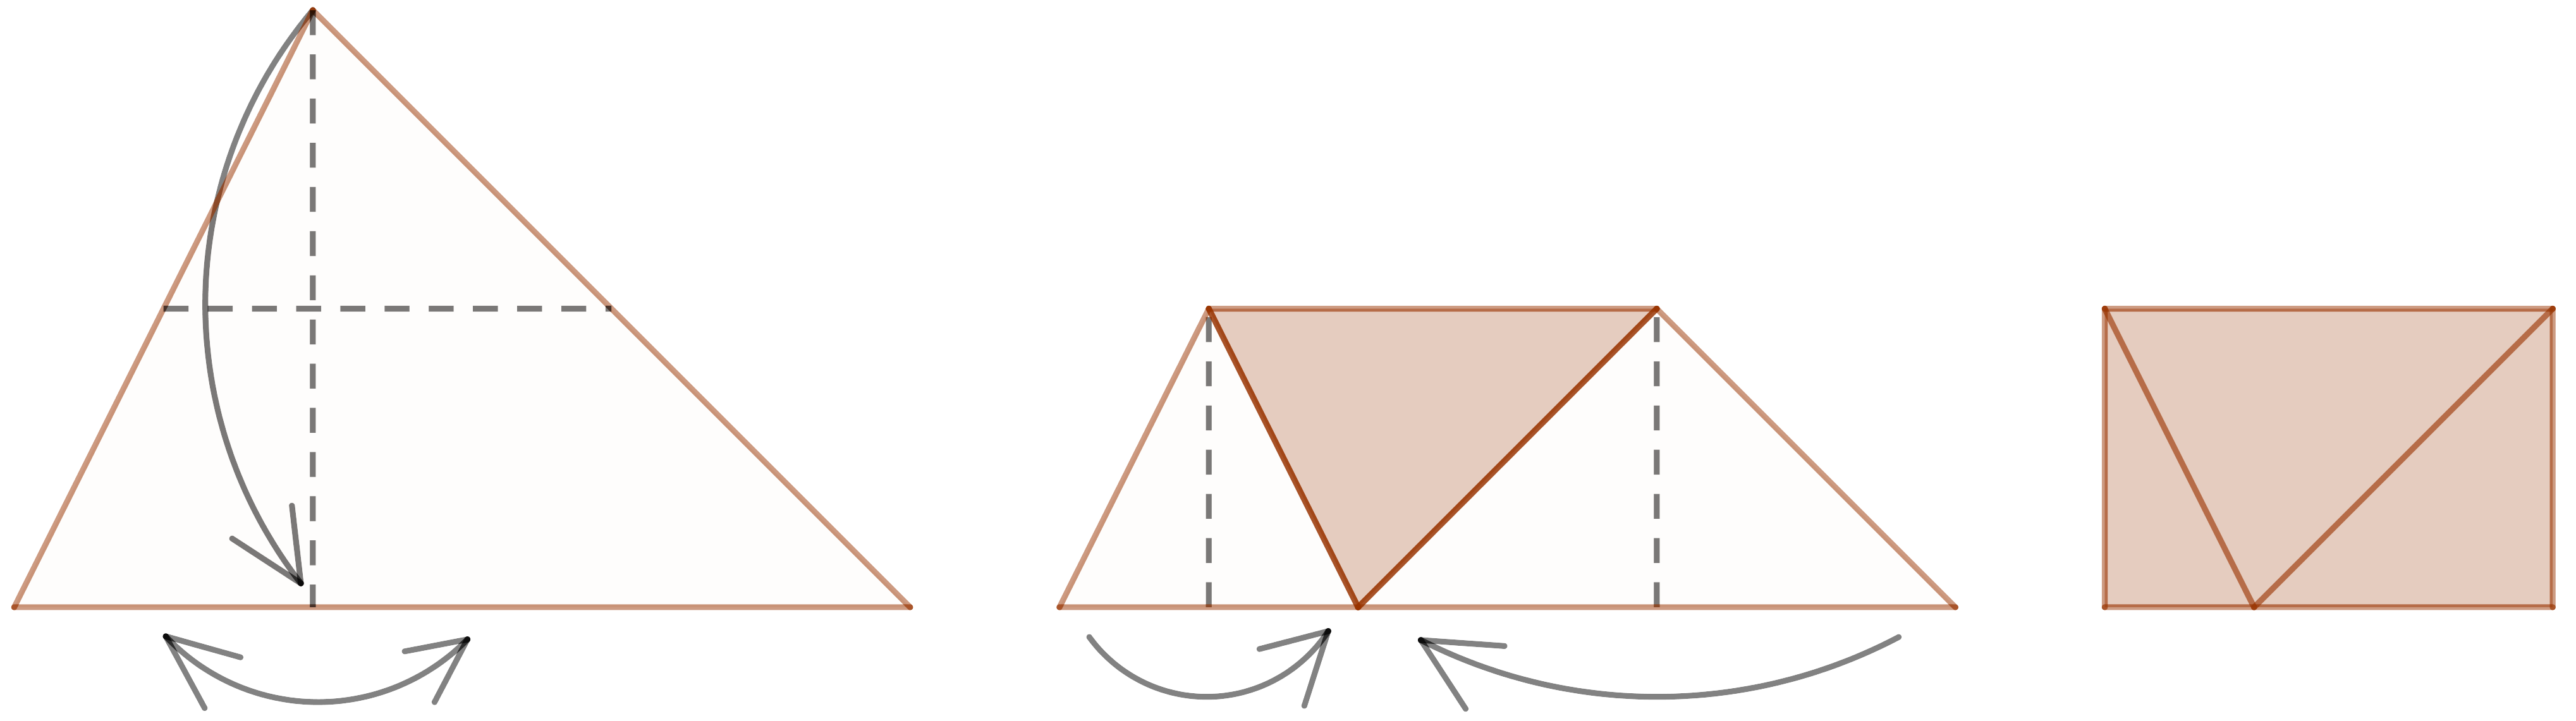
\includegraphics[width=0.8\textwidth]{images/osnovnosolski_prikazi/trikotnik_vsota_kotov.png}
    \caption[Vsota notranjih kotov trikotnika]{Pregib trikotnika, ki njegove notranje kote zloži skupaj v iztegnjeni kot.}
    \label{fig:trikotnik_vsota_kotov}
\end{figure}

Nadalje z določitvijo središča hipotenuze pravokotnega trikotnika bralca povabi, da se s prepogibi prepriča, da nastala točka osnovni trikotnik razdeli na dva enakokraka trikotnika (slika~\ref{fig:trikotnik_vec_lastnosti} levo). Prav tako se lahko s pregibi prepriča, da se višine trikotnika, njegove težiščnice, simetrale stranic ter simetrale kotov sekajo v isti točki (seveda vsaka skupina daljic zase; na sliki~\ref{fig:trikotnik_vec_lastnosti} so prikazani vsi primeri razen za simetralo kotov).

\begin{figure}[h]
    \centering
    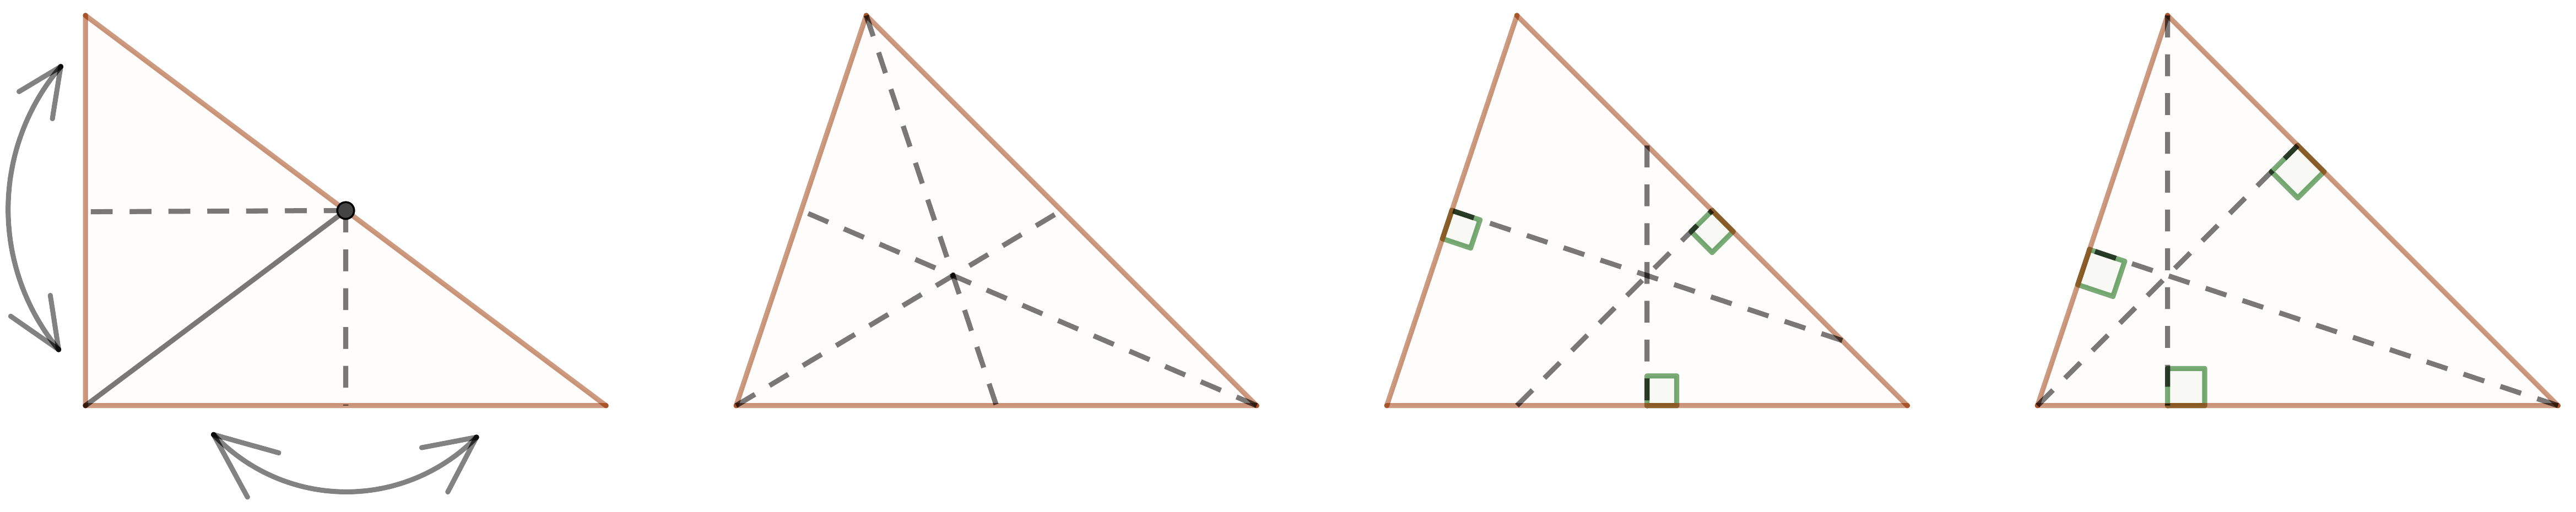
\includegraphics[width=0.95\textwidth]{images/osnovnosolski_prikazi/vec_lastnosti1.png}
    \caption[Pregibi kot dokaz lastnosti trikotnika]{Prikaz še nekaj lastnosti trikotnika.}
    \label{fig:trikotnik_vec_lastnosti}
\end{figure}

Če odložimo trikotnik in v roke vzamemo paralelogram, preko prepogiba po njegovi diagonali vidimo, da diagonale v splošnem ne razpolavljajo notranjih kotov (slika~\ref{fig:par_krog_vec_lastnosti} levo). Slednje velja le za romb, za katerega lahko poleg tega takoj pokažemo še, da sta diagonali pravokotni druga na drugo.

Nato se avtor posveti krogu. Vsak prepogib, ki prekrije njegove robove, ga očitno razdeli na pol in je njegov premer. Dva taka, a različna prepogiba določata središče kroga. Dobi se ga tudi tako, da prepognemo dve različni tetivi in skozi vsako izmed njiju še njeno simetralo, ki se sekata v središčni točki (slika~\ref{fig:par_krog_vec_lastnosti} na sredi). Avtor pri opisovanju konstrukcije ne uporablja izrazov, kot so ``simetrala, tetiva'' ipd., temveč bralec šele po opravljenih prepogibih vidi, da gre za običajne evklidske konstrukcije. Razdelek se konča še s ponazoritvijo Talesovega izreka (slika~\ref{fig:par_krog_vec_lastnosti} desno) in konstrukcijo tangente na krožnico preko pravokotnice na premer.

\begin{figure}[h]
    \centering
    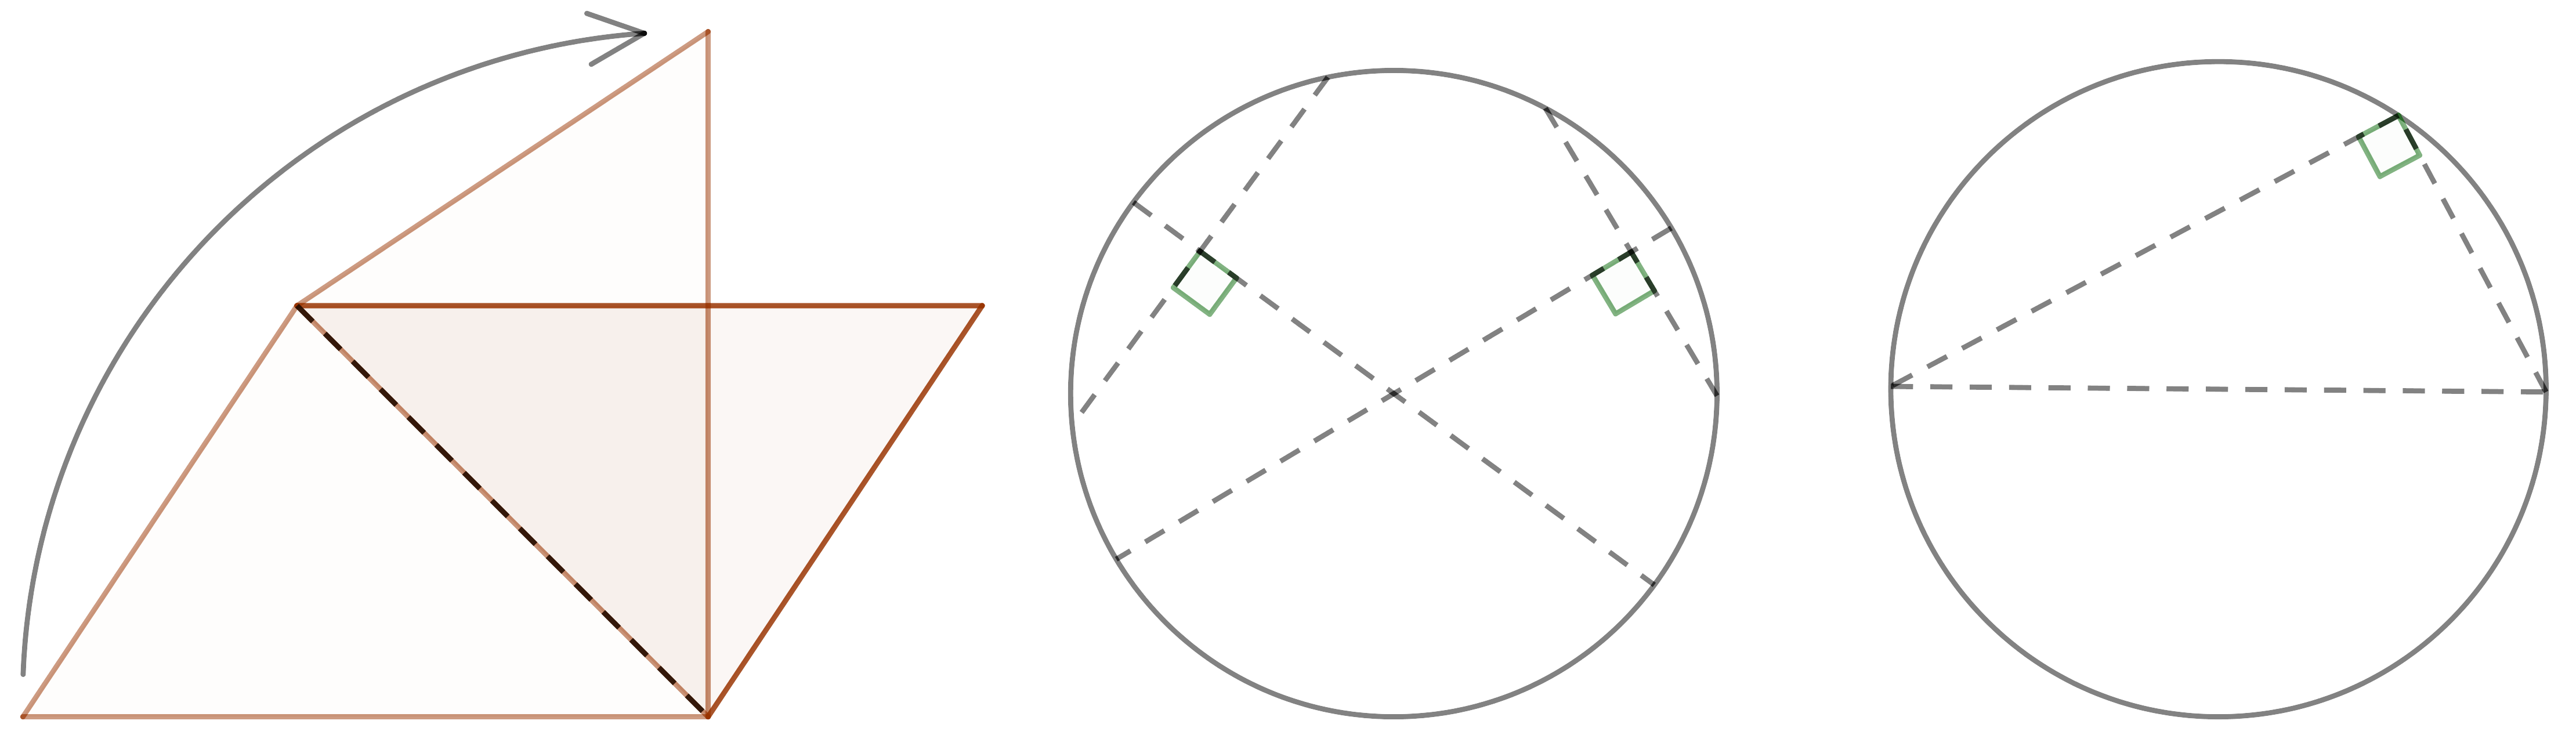
\includegraphics[width=0.9\textwidth]{images/osnovnosolski_prikazi/vec_lastnosti2.png}
    \caption[Pregibi kot dokaz lastnosti paralelograma in kroga]{Prikaz nekaj lastnosti paralelograma in kroga.}
    \label{fig:par_krog_vec_lastnosti}
\end{figure}

Nadalje lahko s prepogibanjem pravokotnika s stranicama $X$ in $X+Y$, kjer krajšo stranico prepognemo na daljšo, ponazorimo odštevanje (slika~\ref{fig:pravok_racunanje} levo). Če nato prepognemo še drugi vogal, dobimo štiri manjše pravokotnike, iz česar lahko bralec sam dokaže formulo $x^2-y^2 = (x-y)(x+y)$ (slika~\ref{fig:pravok_racunanje} desno).

\begin{figure}[h]
    \centering
    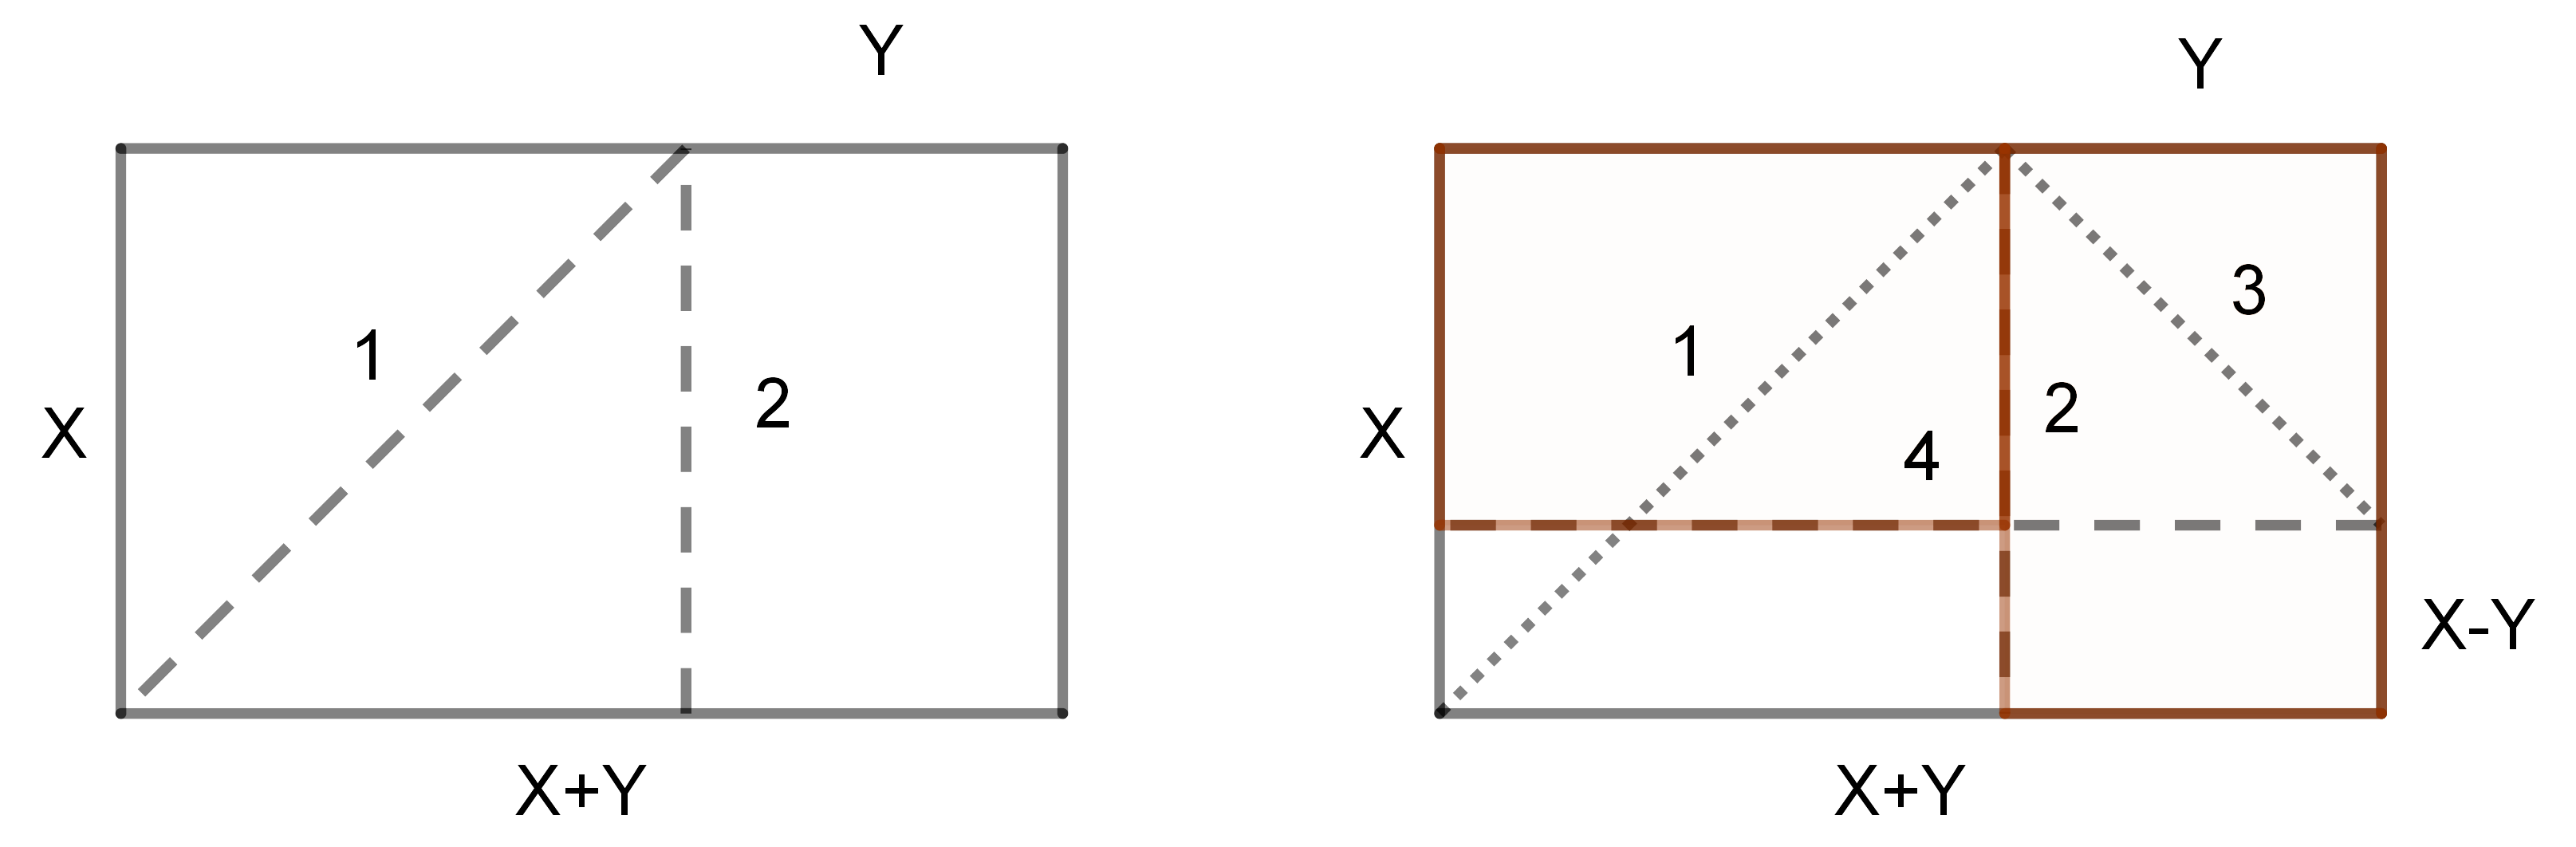
\includegraphics[width=0.8\textwidth]{images/osnovnosolski_prikazi/racunanje.png}
    \caption[Pregibi kot računanje]{Prikaz odštevanja in dokaz formule $x^2-y^2 = (x-y)(x+y)$ z označenim vrstnim redom prepogibov.}
    \label{fig:pravok_racunanje}
\end{figure}

\subsubsection*{Konstrukcija enakostraničnega trikotnika, šestkotnika in osemkotnika}

Trije nevzporedni pregibi, ki se ne sekajo v isti točki, nam na papirju konstruirajo trikotnik. S štirimi pravokotnimi prepogibi dobimo pravokotnik, če njegovo krajšo stranico prepognemo na daljšo, pa še kvadrat (kar smo že storili pri konstrukciji v prejšnjem odstavku). Če njegova oglišča prepognemo v presečišče diagonal, dobimo nov kvadrat s polovično ploščino originalnega.

Konstrukcije poljubnega trikotnika, pravokotnika in kvadrata so zelo enostavne. Malo več premisleka pa je potrebnega za konstrukcije pravilnih $n$-kotnikov. Iz razdelka~\ref{podpogl:n_kotniki} vemo, da je edini pravilni $n$-kotnik, kjer je $n \leq 20$ in se ga ne da konstruirati z origamijem, $11$-kotnik. Postopkov za konstrukcije ostalih večkotnikov je več. Johnson se na primer v nadaljevanju iste knjige posveti konstrukciji preko večkratnega zvijanja traku, kar pa krši pravilo o enkratnih prepogibih papirja.

Pogledali si bomo še origami konstrukcije enakostraničnega trikotnika, šestkotnika in osemkotnika, ki jih navajata Johnson v istem viru~\cite[str.\ 14--15]{johnson1957} in Hull v~\cite[str.\ 1--12]{hull2013}. Iz razdelka~\ref{podpogl:n_kotniki} že vemo, da se jih da konstruirati z evklidskim orodjem, zato bomo v bistvu konstrukcije z ravnilom in šestilom prevedli v konstrukcije s prepogibanjem papirja in ne bomo odkrili ničesar novega.

Vzemimo kvadratni list papirja, ga po višini prepognimo na pol in na pregib položimo spodnje desno oglišče $A$ kvadrata, da nov pregib poteka skozi spodnje levo oglišče $B$ (slika~\ref{fig:trik_enak_basic}). Sliko oglišča $A$ označimo s točko $P$. Ker je po konstrukciji $|AB| = |PB|$ in je vertikalen prepogib simetrala spodnje stranice kvadrata, je trikotnik $\triangle ABP$ enakostraničen.

\begin{figure}[h]
    \centering
    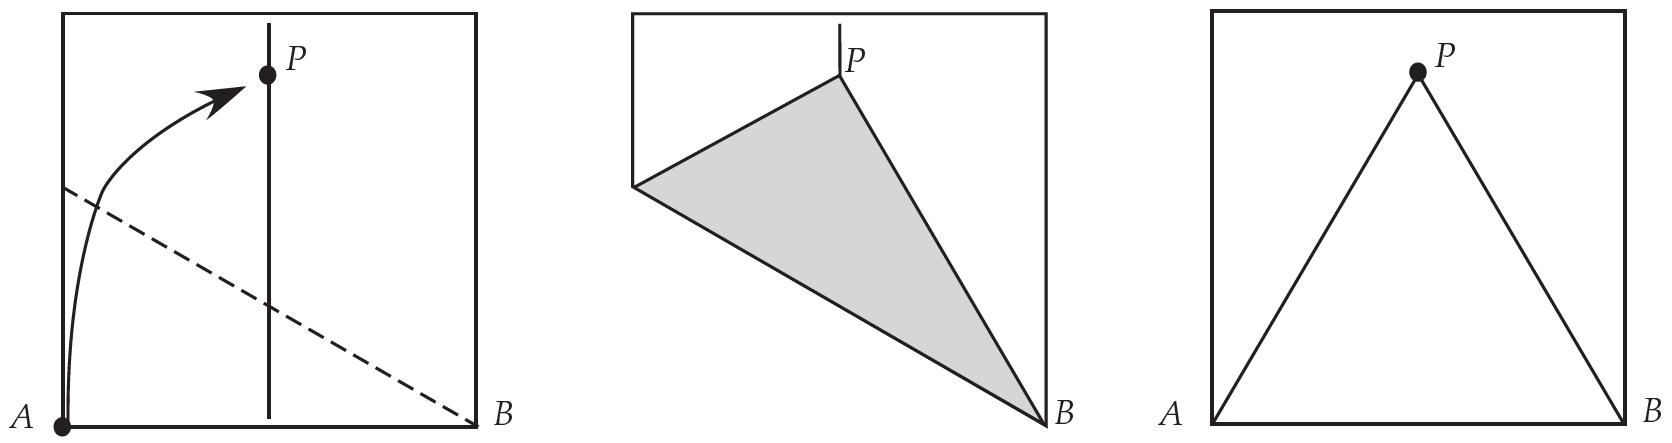
\includegraphics[width=0.9\textwidth]{images/n-kotniki/trik_enak_basic.png}
    \caption[Konstrukcija enakostraničnega trikotnika (način $1$)]{Konstrukcija enakostraničnega trikotnika. Predelano iz~\cite[str. 9]{hull2013}.}
    \label{fig:trik_enak_basic}
\end{figure}

Sedaj, ko znamo konstruirati enakostranične trikotnike, lahko konstruiramo tudi pravilni šestkotnik -- kvadrat s simetralama stranic razdelimo na štiri dele, nato pa v vsakem od štirih manjših kvadratov po zgornjem postopku konstruiramo enakostranični trikotnik (oz. le eno njegovo stranico) z osnovnico na horizontalni simetrali (prve tri figure na sliki~\ref{fig:6kotnik_basic}).

\begin{figure}[h]
    \centering
    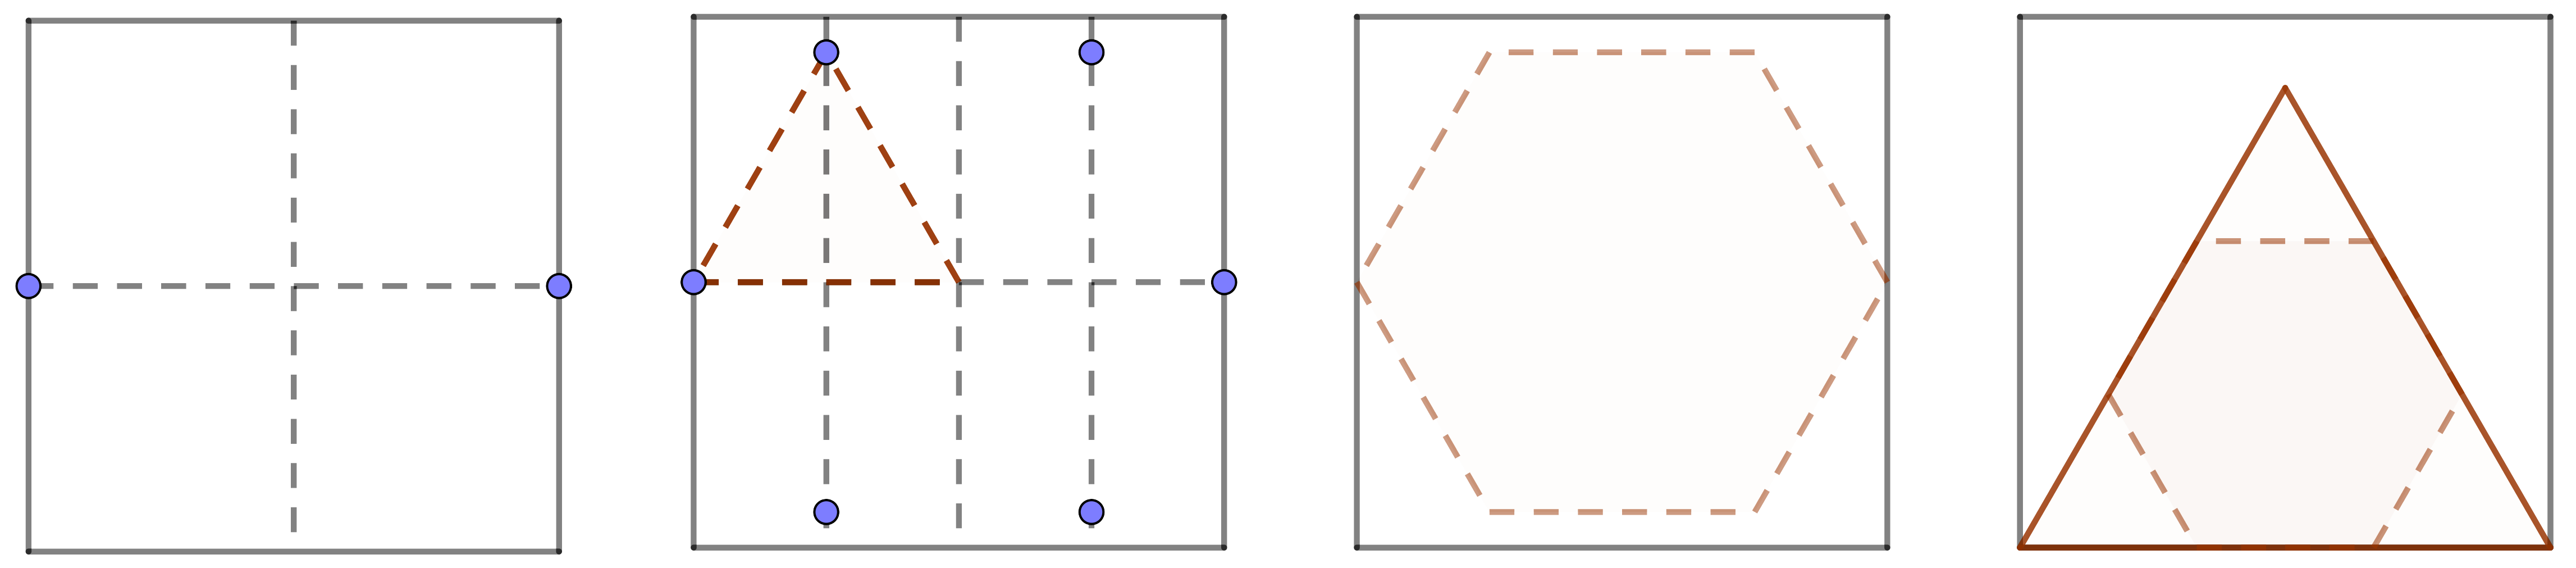
\includegraphics[width=0.95\textwidth]{images/n-kotniki/6kotnik_basic.png}
    \caption[Konstrukcija pravilnega šestkotnika (način $1$) in $2$]{Konstrukcija pravilnega šestkotnika na dva načina.}
    \label{fig:6kotnik_basic}
\end{figure}

Še lažje pravilni šestkotnik konstruiramo preko enakostraničnega trikotnika, ki mu vrhove prepognemo v središče (slika~\ref{fig:6kotnik_basic} desno). Ker središče deli višine v razmerju $2:1$, pregibi stranice razdelijo na tri skladne dele, sam trikotnik pa na tri manjše enakostranične trikotnike in šestkotnik na sredi.

V roke vzemimo nov kvadraten list papirja in konstruirajmo najprej središča njegovih stranic. S pregibi skozi sosednji središči dobimo manjši kvadrat (slika~\ref{fig:8kotnik_basic} levo). Sedaj razpolovimo še vsak kot, ki ima vrh v središču stranice večjega kvadrata in za kraka po eno stranico vsakega kvadrata. Presečišča simetral dveh sosednjih kotov nam dajo še preostala štiri oglišča pravilnega osemkotnika (slika~\ref{fig:8kotnik_basic} desno).

\begin{figure}[h]
    \centering
    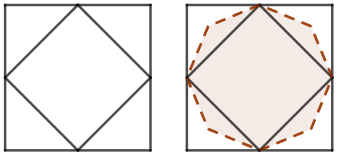
\includegraphics[width=0.6\textwidth]{images/n-kotniki/8kotnik_basic.png}
    \caption[Konstrukcija pravilnega osemkotnika]{Konstrukcija pravilnega osemkotnika.}
    \label{fig:8kotnik_basic}
\end{figure}

Ob oznakah na sliki~\ref{fig:8kotnik_basic} (desno) premislimo, da je to res pravilni osemkotnik: zaradi simetrije so vse stranice skladne, zato moramo dokazati le še skladnost vseh notranjih kotov. Zaradi simetrije je dovolj izračunati notranja kota osemkotnika pri ogliščih $B$ in $C$, ki morata po formuli za notranji kot pravilnega $n$-kotnika oba biti velika $(8-2)/8 \cdot 180^\circ = 135^\circ$. Na sliki je kot $\alpha = 45^\circ /2 = 22{,}5^\circ$, zato je kot ob oglišču $B$ velik $90^\circ + 2\alpha = 135^\circ$, kot ob oglišču $C$ pa izračunamo iz notranjih kotov trikotnika $\triangle ABC$: $\gamma = 180^\circ - 2\alpha = 135^\circ$. Kota sta skladna in ustrezata notranjemu kotu za pravilni osemkotnik.

Vrnimo se nazaj na enakostranični trikotnik v danem kvadratnemu listu papirja. Ali znamo konstruirati največji tak trikotnik -- in če da, kako? Recimo, da obstaja tak trikotnik. Najprej premislimo, da mora vsaj eno njegovo oglišče ležati v oglišču kvadrata. Če to ne drži, se trikotnik ne dotika ene stranice kvadrata -- ker ima tri stranice, kvadrat pa štiri -- recimo spodnje. Potem se z ostalimi tremi oglišči dotika preostalih treh stranic kvadrata, sicer to ne bi bil največji trikotnik -- lahko bi ga še povečali. Potisnimo sedaj trikotnik navzdol po kvadratu, dokler se najnižje oglišče na eni od pokončnih stranic kvadrata ne dotakne njegove spodnje stranice -- kar se zgodi ravno v oglišču kvadrata. Zaradi simetrije brez škode privzemimo, da je to spodnje levo oglišče.

\begin{figure}[h]
    \centering
    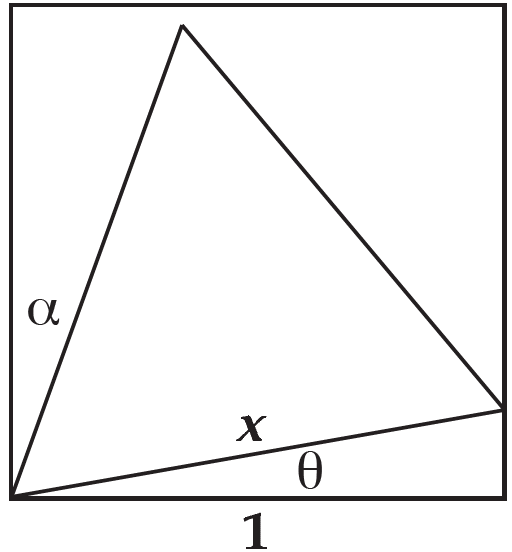
\includegraphics[width=0.25\textwidth]{images/n-kotniki/trik_enak_max1.png}
    \caption[Lega največjega enakostraničnega trikotnika znotraj kvadrata]{Lega največjega enakostraničnega trikotnika znotraj kvadrata.}
    \label{fig:trik_enak_max1}
\end{figure}

Predpostavimo, da ima kvadrat stranico dolžine $1$ in naj bo $\theta$ kot med spodnjima stranicama kvadrata in trikotnika, kot kaže slika~\ref{fig:trik_enak_max1}. Naj bo $x$ dolžina stranice trikotnika. Iščemo tak kot $\theta$, da bo ploščina trikotnika največja. Ker je notranji kot trikotnika velik $60^\circ$, je kot $\theta$ zaradi simetrije omejen z $0 \leq \theta \leq 15^\circ$. Ob upoštevanju $x = 1/ \cos \theta$ je njegova ploščina
$$ P = \frac{\sqrt{3}}{4} x^2 = \frac{\sqrt{3}}{4} \cdot \frac{1}{\cos^2 \theta}. $$
Funckijo bi lahko odvajali in preko iskanja njenega maksimuma izrazili kot, Hull pa v~\cite[str.\ 11]{hull2013} predlaga enostavnejšo rešitev. Ker je $\cos x$ na intervalu $[0^\circ, 15^\circ]$ oz.\ $[0, \pi/12]$ pozitivna in padajoča, je njena obratna vrednost naraščajoča, zato je tudi $1/\cos^2\theta$ naraščajoča funkcija. Ploščina $P(\theta)$ torej narašča in maksimum doseže pri $\theta = 15^\circ$.

Trikotnik je simetričen glede na diagonalo kvadrata. Na sliki~\ref{fig:trik_enak_max2} (levo) je prikazana konstrukcija kota $15^\circ$ -- spodnje belo območje enakostraničen trikotnik in vsak od pregibov je simetrala kota $30^\circ$. Če opravimo taka dva pregiba na sosednjih stranicah, kot kaže slika~\ref{fig:trik_enak_max2} na sredi, tako dobimo iskani največji enakostranični trikotnik v danem kvadratu.

\begin{figure}[h]
    \centering
    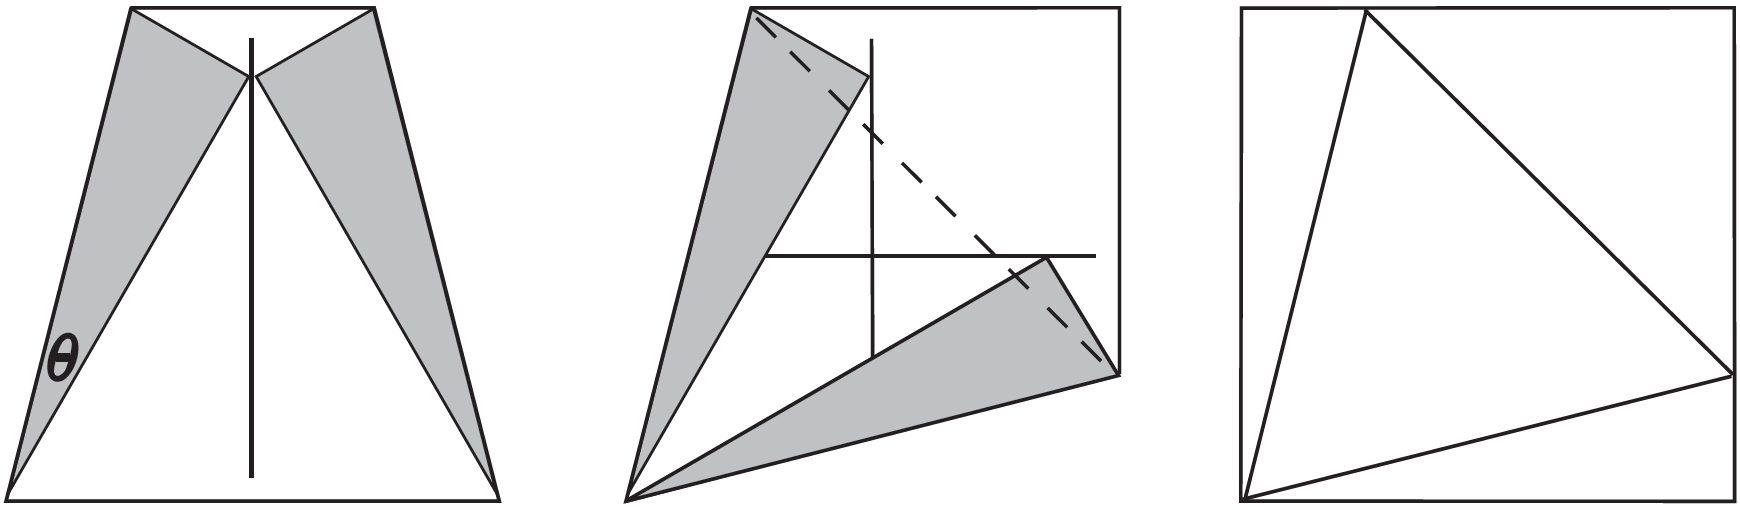
\includegraphics[width=0.8\textwidth]{images/n-kotniki/trik_enak_max2.png}
    \caption[Konstrukcija največjega enakostraničnega trikotnika znotraj kvadrata]{Konstrukcija največjega enakostraničnega trikotnika znotraj kvadrata.}
    \label{fig:trik_enak_max2}
\end{figure}

\subsection{Hagovi izreki za prepogibanje kvadrata}

S prepogibanjem kvadratnega lista papirja se je veliko ukvarjal Kazuo Haga, sicer japonski profesor biologije. V svojem delu \emph{Origamics: Mathematical Explorations Through Paper Folding}~\cite{haga2008} je tako med drugim formuliral tri izreke, ki jih poznamo pod imenom \emph{Hagovi izreki}. Pri vsakem od njih gre za konstrukcijo specifičnega pregiba, ki povzroči delitev stranic kvadrata v različnih razmerjih. Vsak izrek posebej bomo najprej formulirali, si slikovno ogledali konstrukcijo in ga dokazali, nato pa si pogledali še nekaj dodatnih lastnosti, ki sledijo iz njega.

Da si olajšamo računanje, predpostavimo, da ima kvadrat, ki predstavlja naš list papirja, stranico dolžine $1$. Njegova oglišča označimo s črkami $A, B, C$ in $D$, začenši v zgornjem desnem oglišču in sledečimi v pozitivni smeri, torej nasprotni smeri urinega kazalca.

\subsubsection{Prvi Hagov izrek}

\begin{izrek}[Prvi Hagov izrek]
    Zgornjo stranico $AD$ kvadrata $ABCD$ razpolovimo v točki $E$ in s pregibom nanjo položimo oglišče $C$. S tem na levi in desni stranici kvadrata dobimo tri točke, ki jih označimo z $F, G$ in $H$ (slika~\ref{fig:hagov_izrek1}). Za te točke velja:
    \begin{itemize}
        \item točka $F$ deli desno stranico v razmeru $3:5$,
        \item točka $H$ deli levo stranico v razmerju $2:1$,
        \item če točko $H$ zrcalimo čez pregib na spodnjo stranico, jo deli v razmerju $1:5$,
        \item točke $G$ deli levo stranico v razmerju $7:1$.
    \end{itemize}
\end{izrek}

\begin{figure}[h]
    \centering
    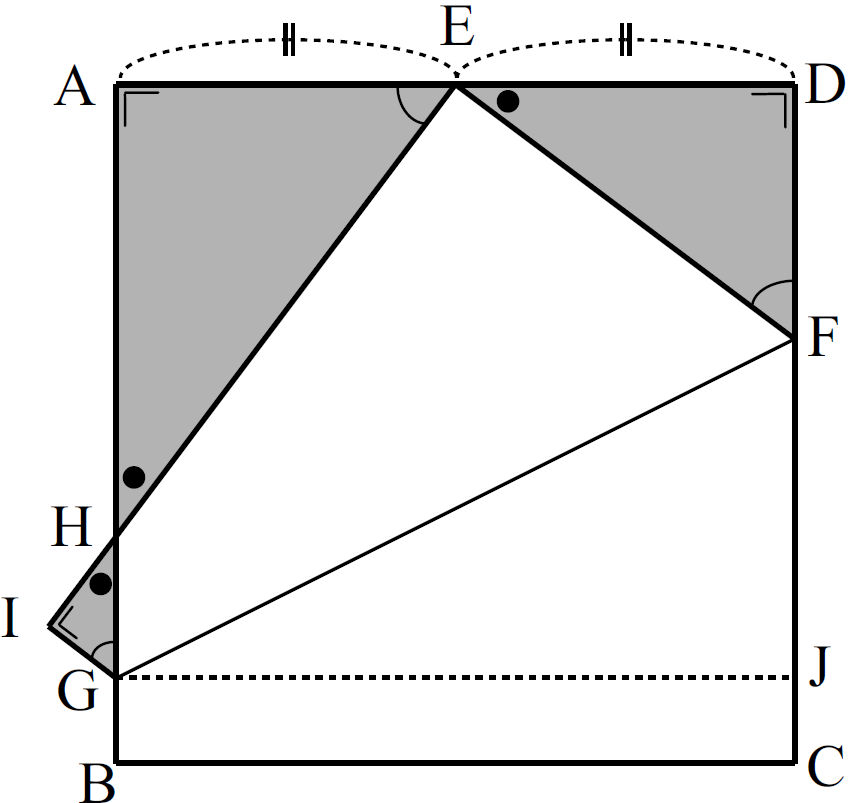
\includegraphics[width=0.4\textwidth]{images/hagovi_izreki/hagov_izrek1.png}
    \caption[Pregib iz prvega Hagovega izreka]{Konstrukcija pregiba iz prvega Hagovega izreka. Vzeto iz~\cite[str. 4]{haga2008}.}
    \label{fig:hagov_izrek1}
\end{figure}

\begin{dokaz}
    Kot kaže slika~\ref{fig:hagov_izrek1}, označimo še točki $I$ in $J$. Najprej lahko opazimo, da pregib iz izreka povzroči nastanek treh podobnih pravokotnih trikotnikov, ki so na sliki~\ref{fig:hagov_izrek1} pobarvani sivo. Za vsakega od njih lahko določimo dolžine njegovih stranic.

    Začnimo s trikotnikom $\triangle DEF$. Ker je $E$ razpolovišče stranice $AD$, je $|DE| = 1/2$. Če drugo kateto $DF$ označimo z $a$, je hipotenuza $EF$ dolga $1-a$, saj $|DF| + |EF| = |DF| + |FC| = 1$ po konstrukciji. Iz Pitagorovega izreka nato izračunamo $a = 3/8$. Torej točka $F$ res deli stranico $CD$ v razmerju $3:5$.

    Iz razmerja podobnih trikotnikov $\triangle DEF$ in $\triangle AHE$ dobimo
    $$ \frac{|AH|}{|AE|} = \frac{|DE|}{|DF|}, \; \text{ torej } \; |AH| = \frac{|AE|\cdot|DE|}{|DF|} = \frac{1/2 \cdot 1/2}{3/8} = \frac{2}{3}.$$
    Točka $H$ res deli stranico $AB$ v razmerju $2:1$. Drugače povedano -- s prvim Hagovim izrekom znamo poljubno daljico razdeliti na tri skladne dele.

    Sedaj lahko izračunamo dolžino hipotenuze $EH$ trikotnika $\triangle AHE$. Iz Pitagorovega izreka sledi $|EH| = 5/6$ (in posledično iz $|EI| = 1$ še $|HI| = 1/6$), torej točka $H$ res deli spodnjo stranico v razmerju $1:5$.

    Za izračun dolžine daljice $BG$, ki je po konstrukciji enaka dolžini katete $GI$, si spet pomagamo z razmerji podobnih trikotnikov; tokrat vzamemo trikotnika $\triangle IHG$ in $\triangle AHE$. Iz razmerja
    $$ \frac{|GI|}{|HI|} = \frac{|AE|}{|AH|} \; \text{ sledi } \; |BG| = |GI| = \frac{|AE|\cdot|HI|}{|AH|} = \frac{1/2 \cdot 1/6}{2/3} = \frac{1}{8},$$
    torej točka $G$ res deli stanico $AB$ v razmerju $7:1$.
\end{dokaz}

Za vajo lahko izračunamo še preostale dolžine daljic:
\begin{align*}
    |GH| &= |AB| - |AH| - |BG| = 1 - \frac{2}{3} - \frac{1}{8} = \frac{5}{24},\\
    |CJ| &= |BG| = \frac{1}{8},\\
    |FJ| &= |CD| - |DF| - |CJ| = 1 - \frac{3}{8} - \frac{1}{8} = \frac{1}{2},\\
    |FG| &= \sqrt{|GJ|^2 + |FJ|^2} = \sqrt{1^2 + \left(\frac{1}{2}\right)^2} = \frac{\sqrt{5}}{2}.
\end{align*}

S tem so znane vse dolžine daljic, na katere pregib iz prvega Hagovega izreka razdeli stranice enotskega kvadrata. Na sliki~\ref{fig:hagov_izrek1_st} je tako povzetek naših ugotovitev.

\begin{figure}[h]
    \centering
    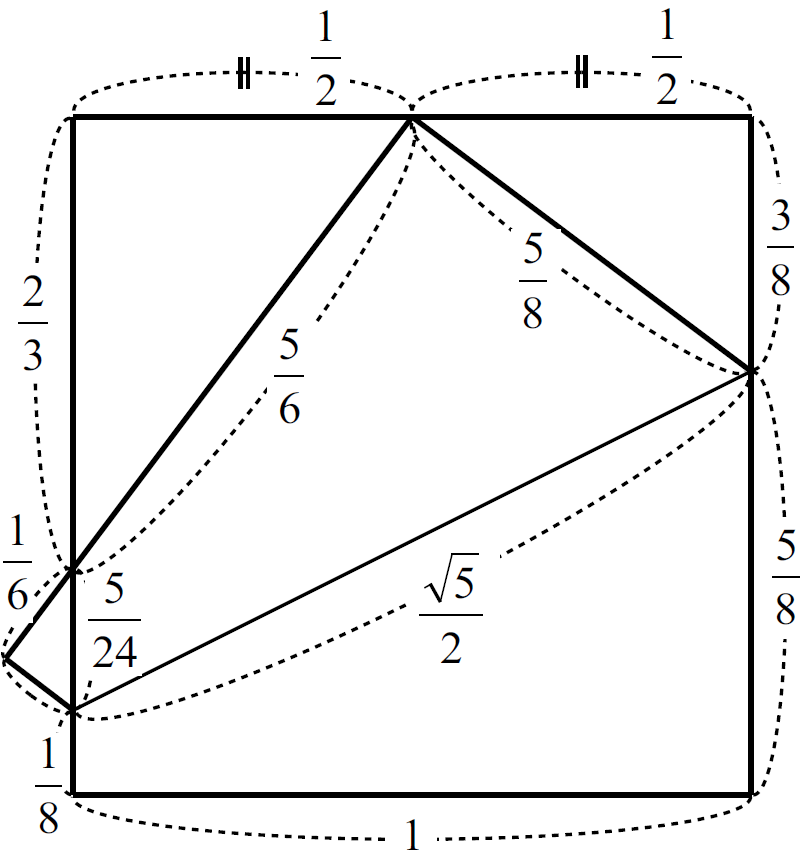
\includegraphics[width=0.4\textwidth]{images/hagovi_izreki/hagov_izrek1_stevilke.png}
    \caption[Prvi Hagov izrek v številkah]{Dolžine daljic po prvem Hagovem izreku. Vzeto iz~\cite[str. 7]{haga2008}.}
    \label{fig:hagov_izrek1_st}
\end{figure}

Izrek lahko tudi posplošimo, če za točko $E$ ne vzamemo razpolovišča, temveč poljubno točko na daljici $AD$. Naj bo $x = |ED|$. Nastale točke označimo kot prej, dolžine nastalih daljic pa z $y_1$ do $y_6$, kot kaže slika~\ref{fig:hagov_izrek1_splosen}.

\begin{figure}[h]
    \centering
    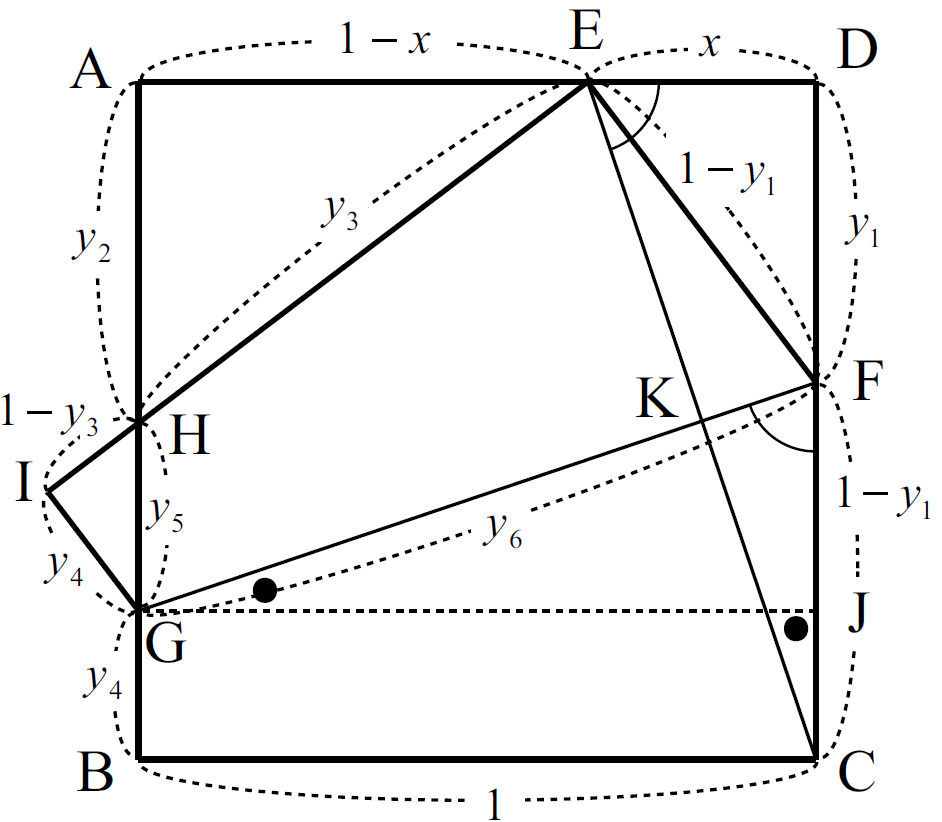
\includegraphics[width=0.5\textwidth]{images/hagovi_izreki/hagov_izrek1_splosen.png}
    \caption[Prvi Hagov izrek v splošnem]{Oznake dolžin iz prvega Hagovega izreka v splošnem. Vzeto iz~\cite[str. 9]{haga2008}.}
    \label{fig:hagov_izrek1_splosen}
\end{figure}

Za vsak $i \in \{1,2,3,4,5,6\}$ poiščimo sedaj vrednost $y_i$ v odvisnosti od $x$. Kot prej najprej opazimo, da imamo zopet tri podobne pravokotne trikotnike. Iz Pitagorovega izreka za pravokotni trikotnik $\triangle EDF$ sledi
$$y_1 = (1-x^2)/2,$$
iz razmerja podobnih pravokotnih trikotnikov $\triangle EDF$ in $\triangle HAE$ pa izračunamo
$$ y_2 = \frac{x(1-x)}{y_1} = \frac{2x}{1+x} \; \text{ in } \; y_3 = \frac{(1-y_1)(1-x)}{y_1} = \frac{1+x^2}{1+x}.$$
Pregib $FG$ je po konstrukciji simetrala daljice $CE$, torej pravokotna nanjo, iz česar sledi, da sta trikotnika $\triangle CKF$ in $\triangle CDE$ podobna in kota $\angle DEC$ in $\angle KFC$ skladna. Zato sta skladna tudi trikotnika $\triangle CDE$ in $\triangle GJF$, torej $|FJ| = x$. Posledično je
$$y_4 = |CJ| = 1 - (y_1 + x) = \frac{(1-x)^2}{2} \; \text{ in } \; y_5 = 1 - y_2 - y_4 = \frac{(1-x)(1+x^2)}{2(1+x)}.$$
Na koncu še s ponovno uporabo Pitagorovega izreka izračunamo
$$ y_6 = \sqrt{|GJ|^2 + |FJ|^2} = \sqrt{1 + x^2}.$$

Splošne vrednosti dolžin $y_i$ mogoče niso najlepše, vendar pri marsikateri izbiri števila $x \in (0,1)$ dobimo lepe številke. Najbolj so zanimiva recipročna števila naravnih števil. Vemo že, da pri izbiri $x = 1/2$ lahko dobimo števila $1/3, 1/6, 1/8$, pri izbiri $x = 1/4$ in $x = 3/4$ dobimo še $2/5$ (in iz tega z razpolovitvijo $1/5$) in $1/7$. Računanje prepuščamo bralcu, se pa na tej točki lahko vprašamo, ali za vsak $n \in \N$ obstaja primeren $x$, da lahko preko neke dolžine $y_i$ ali $1-y_i$ in preko postopkov za konstrukcijo že znanih razmerij konstruiramo dolžino $1/n$. Odgovor je pritrdilen, enostaven razmislek pa sledi v razdelku~\ref{podpogl:razdelitev_hag1_spl}.

\subsubsection{Drugi Hagov izrek}

\begin{izrek}[Drugi Hagov izrek]
    Zgornjo stranico $AD$ kvadrata $ABCD$ razpolovimo v točki $E$ in opravimo pregib skozi točko $E$ ter oglišče $C$. Točka $D$ se tako preslika v točko $F$ (slika~\ref{fig:hagov_izrek2}). Če stranico $EF$ podaljšamo do leve stranice kvadrata, jo presečišče $G$ razdeli v razmerju $2:1$.
\end{izrek}

\begin{figure}[h]
    \centering
    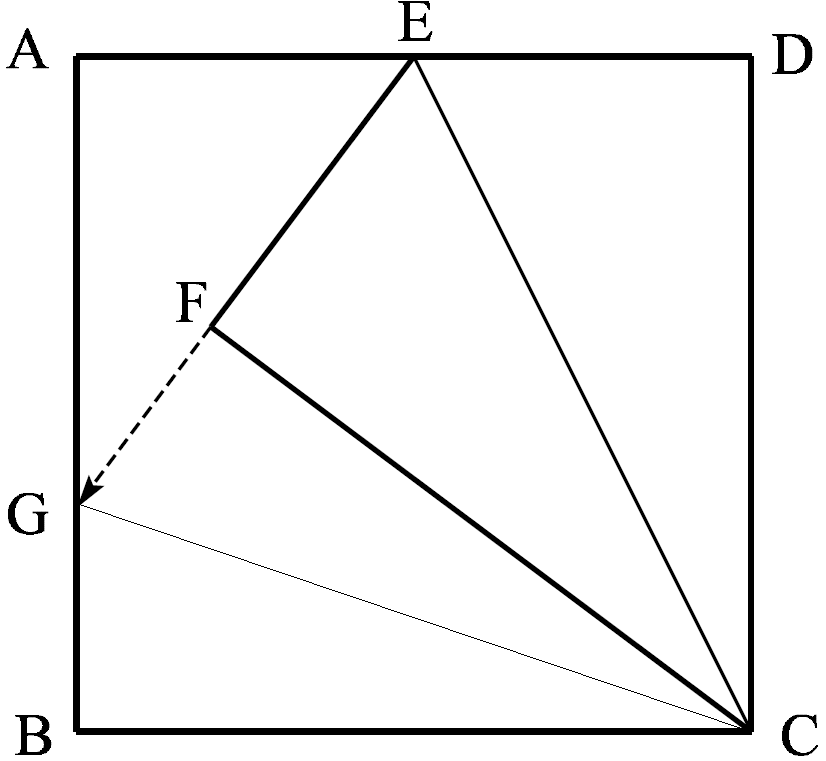
\includegraphics[width=0.4\textwidth]{images/hagovi_izreki/hagov_izrek2.png}
    \caption[Pregib iz drugega Hagovega izreka]{Konstrukcija pregiba iz drugega Hagovega izreka. Vzeto iz~\cite[str. 12]{haga2008}.}
    \label{fig:hagov_izrek2}
\end{figure}

\begin{dokaz}
    Opazimo lahko, da sta trikotnika $\triangle BCG$ in $\triangle FCG$ skladna, saj imata skladni daljšo kateto in hipotenuzo ter pravi kot nasproti hipotenuze. Označimo $x = |GB| = |GF|$. Zapišimo Pitagorov izrek za pravokotni trikotnik $\triangle AGE$:
    $$ \left(x + \frac{1}{2}\right)^2 = (1-x)^2 + \left(\frac{1}{2}\right)^2 \; \text{ in izračunamo } \; x = \frac{1}{3},$$
    torej točka $G$ res deli stranico $AB$ v razmerju $2:1$.
\end{dokaz}

S tem smo zopet dobili način razdelitve daljice na tri enake dele, a tu zanimivih razmerij še ni konec. Poglejmo si še, v kakšen razmerju nam stranice deli točka $F$ in točke, ki jih dobimo s podaljšanjem daljic $FD$ in $FC$ do leve stranice. Označimo nove točke $H, I, J, K$ in $M$, kot kaže slika~\ref{fig:hagov_izrek2_st}.

\begin{figure}[h]
    \centering
    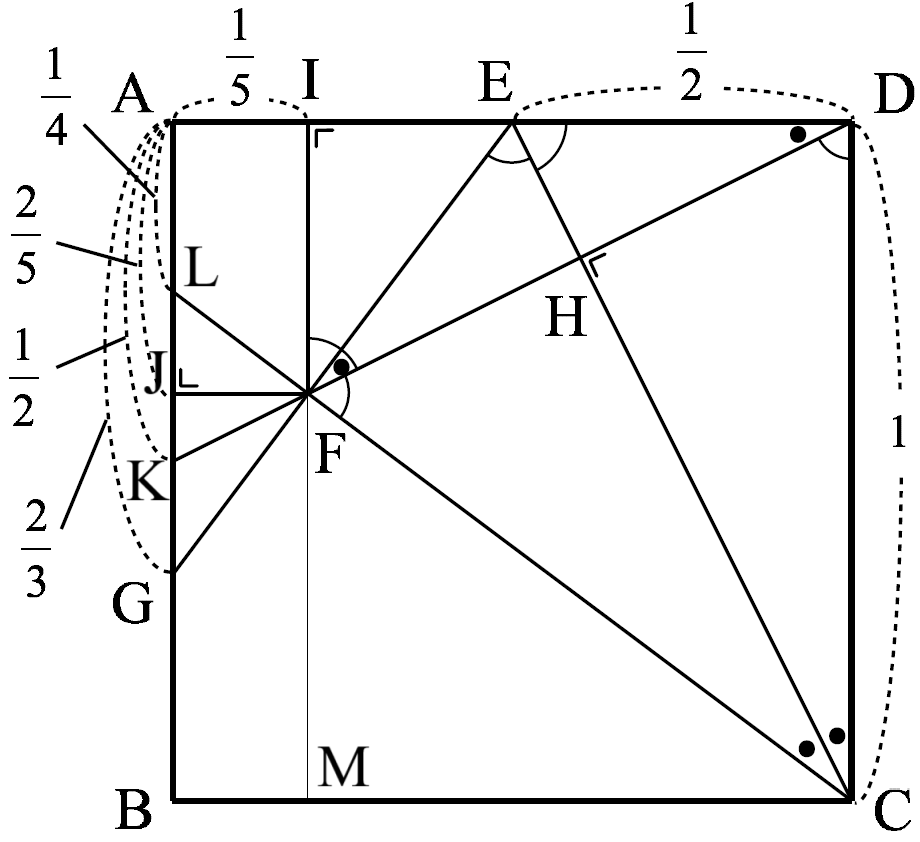
\includegraphics[width=0.45\textwidth]{images/hagovi_izreki/hagov_izrek2_stevilke.png}
    \caption[Drugi Hagov izrek v številkah]{Razdalje po drugem Hagovem izreku. Preurejeno iz~\cite[str. 15]{haga2008}.}
    \label{fig:hagov_izrek2_st}
\end{figure}

Po konstrukciji pregiba velja $FD \perp CE$, iz česar dobimo podobne pravokotne trikotnike $\triangle CDE$, $\triangle CFE$, $\triangle DAK$, $\triangle DHE$, $\triangle FHE$, $\triangle DIF$. Prvi trije od naštetih so celo skladni, prav tako je skladen tudi sledeči par. Le trikotnik $\triangle DIF$ nima skladnega para. Iz sledečih razmerij izračunamo
\begin{align*}
    |DH| &= \frac{|DE| \cdot |CD|}{|CE|} = \frac{1}{\sqrt{5}}, \; \text{ torej } \; |DF| = 2|FH| = \frac{2}{\sqrt{5}}, \\
    |DI| &= \frac{|DF| \cdot |CD|}{|CE|} = \frac{4}{5}, \; \text{ torej } \; |AI| = \frac{1}{5}, \\
    |FI| &= \frac{|DI| \cdot |DE|}{|CD|} = \frac{2}{5} \; \text{ in} \\
    |AK| &= |DE| = \frac{1}{2}.
\end{align*}

Iz podobnih trikotnikov $\triangle BCL$ in $\triangle MCF$ sledi še
$$ |BL| = \frac{|BC| \cdot |FM|}{|CM|} = \frac{3}{4}, \; \text{ torej } \; |AL| = |AB| - |BL| = \frac{1}{4}. $$

Torej nam drugi Hagov izrek poleg konstrukcije števil $1/3, 2/3$ poda tudi diretkno konstrukcijo števil $1/5, 2/5, 3/5$ in $4/5$.

\subsubsection{Tretji Hagov izrek}

\begin{izrek}[Tretji Hagov izrek]
    Zgornjo stranico $AD$ kvadrata $ABCD$ razpolovimo v točki $E$ in opravimo pregib, ki točko $E$ položi na desno stranico in hkrati oglišče $C$ na levo stranico (slika~\ref{fig:hagov_izrek3}). Njena slika $H$ levo stranico deli v razmerju $2:1$.
\end{izrek}

\begin{figure}[h]
    \centering
    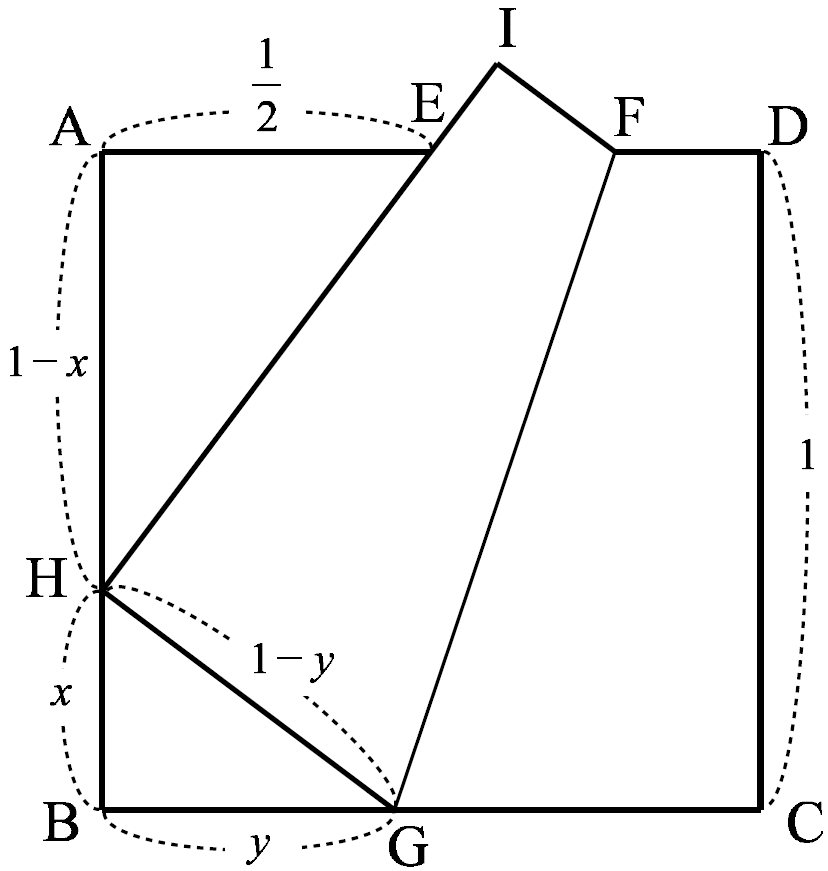
\includegraphics[width=0.4\textwidth]{images/hagovi_izreki/hagov_izrek3.png}
    \caption[Pregib iz tretjega Hagovega izreka]{Konstrukcija pregiba iz tretjega Hagovega izreka. Vzeto iz~\cite[str. 18]{haga2008}.}
    \label{fig:hagov_izrek3}
\end{figure}

\begin{dokaz}
    Označimo še točke $E, F, G,$ in $I$ ter uvedimo $x = |BH|$ in $y = |BG|$, kot kaže slika~\ref{fig:hagov_izrek3}. Zaradi prepogiba je $|GH| = |CG| = 1-y$. Iz Pitagorovega izreka za pravokotni trikotnik $\triangle BGH$ ter razmerja za podobna trikotnika $\triangle BGH$ in $\triangle AHE$ dobimo sistem enačb
    $$ x^2 + y^2 = (1-y)^2 \; \text{ in } \; \frac{1/2}{1-x} = \frac{x}{y}, $$
    iz katerih izračunamo $x = \frac{1}{3}$ in $y = \frac{4}{9}$. Torej točka $H$ res deli stranico $AB$ v razmerju $2:1$.
\end{dokaz}

Kot pri prejšnjih dveh izrekih bi lahko poračunali še preostale dolžine daljic. To za vajo prepuščamo bralcu, ki se lahko o svojih rezultatih prepriča s sliko~\ref{fig:hagov_izrek3_st}.

\begin{figure}[h]
    \centering
    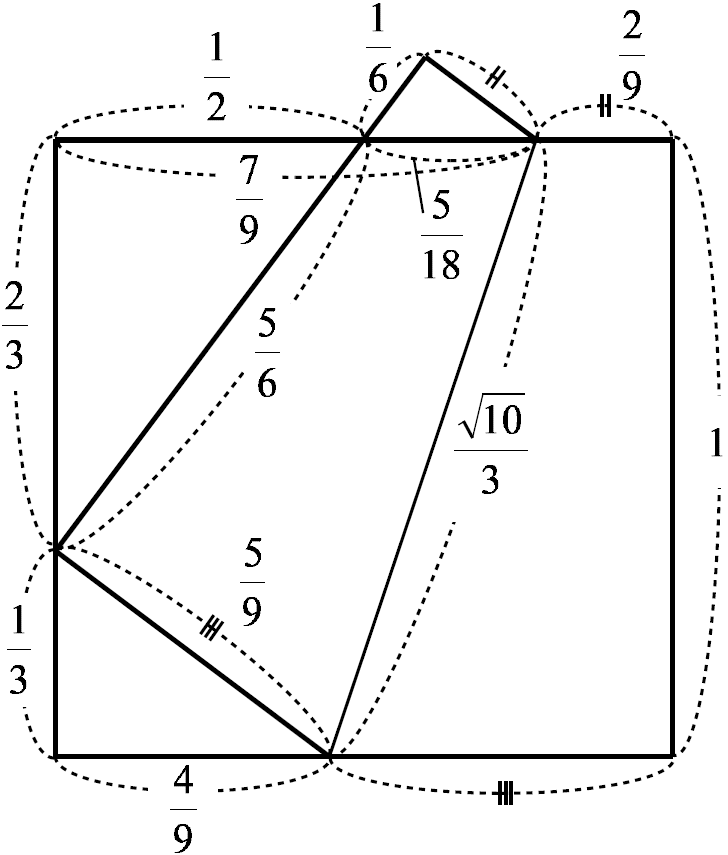
\includegraphics[width=0.4\textwidth]{images/hagovi_izreki/hagov_izrek3_stevilke.png}
    \caption[Tretji Hagov izrek v številkah]{Dolžine daljic po tretjem Hagovem izreku. Vzeto iz~\cite[str. 19]{haga2008}.}
    \label{fig:hagov_izrek3_st}
\end{figure}

Pri vseh treh Hagovih izrekih gre torej za prepogib, ki ali gre skozi središče zgornje stranice $AD$ ali stranico $CD$ kvadrata $ABCD$ položi nanj. V vsakem primeru nam konstrukcija poda točko na levi stranici $AB$, ki jo deli v razmerju $2:1$, torej sedaj zmoremo (na več načinov) poljubno daljico razdeliti na tri skladne dele. Če popustimo pogoj, da uporabljamo središče stranice $AD$, lahko z izbiro poljubne točke na tej stranici kvadrata izreke posplošimo in dobimo več zanimivih razmerij, kot se izkaže, celo razmerje $n:1$ za poljuben $n \in \N$.

Avtor Haga je svoje izreke preizkusil tudi na \emph{srebrnih pravokotnikih}\footnote{To so pravokotniki, ki imajo stranice v razmerju $1 : \sqrt{2}$. Lastnost tega razmerja je, da če tak pravokotnik prepoloviš po daljši stranici, dobiš nov, za pol manjši srebrni pravokotnik. Primer takega pravokotnika je kar A4 list papirja -- prepričaš se lahko tako, da krajšo stranico prepogneš na daljšo, da dobiš diagonalo kvadrata, in preveriš, da je ta pregib enako dolg kot daljša stranica. To je enak princip kot pri zlatih pravokotnikih, kjer je razmerje stranic v zlatem rezu.} in tako prišel do novih načinov razdelitev na 9, 14, 16 in še več različnih delov. Tu se s tem ne bomo ukvarjali, zato naj si bralec, ki ga zanima več, to pogleda v~\cite[str.\ 21--32]{haga2008}.

\subsection{Razdelitev daljice na $n$ skladnih delov}

Stranico kvadrata želimo razdeliti na $n$ enakih delov, kjer je $n \in \N$ poljuben. Za $n = 2^t$, kjer je $t \in \N_0$, je to čisto enostavno, saj samo prepolavljamo razdalje med pregibi, dokler ne dosežemo cilja. Če je $n$ sod, vendar ni potenca števila $2$, torej $n = 2^t(2m + 1)$, kjer sta $t, m \in \N$, stranico najprej razdelimo na $2^t$ delov, nato pa moramo vsakega izmed njih razdeliti na $2m + 1$ (liho število) delov. Izziv tega problema je torej v razdelitvi daljice na liho število delov. Ko bomo to zmogli, jo bomo znali razdeliti na $n$ delov za vsak $n \in \N$.

V prejšnjem razdelku so nam Hagovi izreki podali razdelitev stranice kvadrata na tri, pet, sedem in devet delov. Vendar iščemo metodo, ki nam stranico razdeli na $n$ delov za splošen lih $n \in \N$. Spomnimo se, da smo en tak postopek že spoznali -- v dokazu izreka~\ref{izr:podpolje} smo za poljuben $a \in \R$ znali konstruirati razdaljo $1/a$, kar bi lahko uporabili za razdelitev neke daljice na $a$ enakih delov -- konstruirano razdaljo $1/a$ bi $a$-krat prenesli naprej. Načinov reševanja tega problema pa se je skozi zadnja desetletja oblikovalo še veliko več; tu bomo spoznali še dve metodi.

\subsubsection*{Metoda po posplošenem prvem Hagovem izreku}
\label{podpogl:razdelitev_hag1_spl}

Spomnimo se prvega Hagovega izreka, kjer nam prepogib oglišča $B$ na središče daljice $AD$ v točki $H$ na daljici $AB$ povzroči njeno razdelitev v razmerju $2:1$. Nato smo izrek posplošili in namesto središča zgornje stranice izbrali poljubno točko, ki je za $x$ odmaknjena od oglišča $D$ (slika~\ref{fig:hagov_izrek1_splosen}). Pri tem smo med drugim izračunali razdaljo $y_2 = |HA| = 2x/(1+x)$.

Razveseli nas, da pri $x = 1/n$ dobimo ravno $y_2 = 2/(n+1)$, kar je dvakratnik števila $1/(n+1)$. Če torej znamo zgornjo stranico razdeliti v razmerju $(n-1):1$, nam središče daljice $HA$ levo stranico razdeli v razmerju $n:1$. Na sliki~\ref{fig:razdelitev_daljice_h1} je prikaz za $n = 2, 3, 4$ in splošen $n$ (pri tem se sicer na zgornjo stranico prepogne spodnje levo oglišče, zato je to zrcalna različica slike, kot smo je vajeni). Po indukciji (prvi Hagov izrek je baza indukcije pri $n=2$) je to še ena metoda za razdelitev daljice na poljubno število skladnih delov preko prepogibanja kvadratnega lista papirja.

\begin{figure}[h]
    \centering
    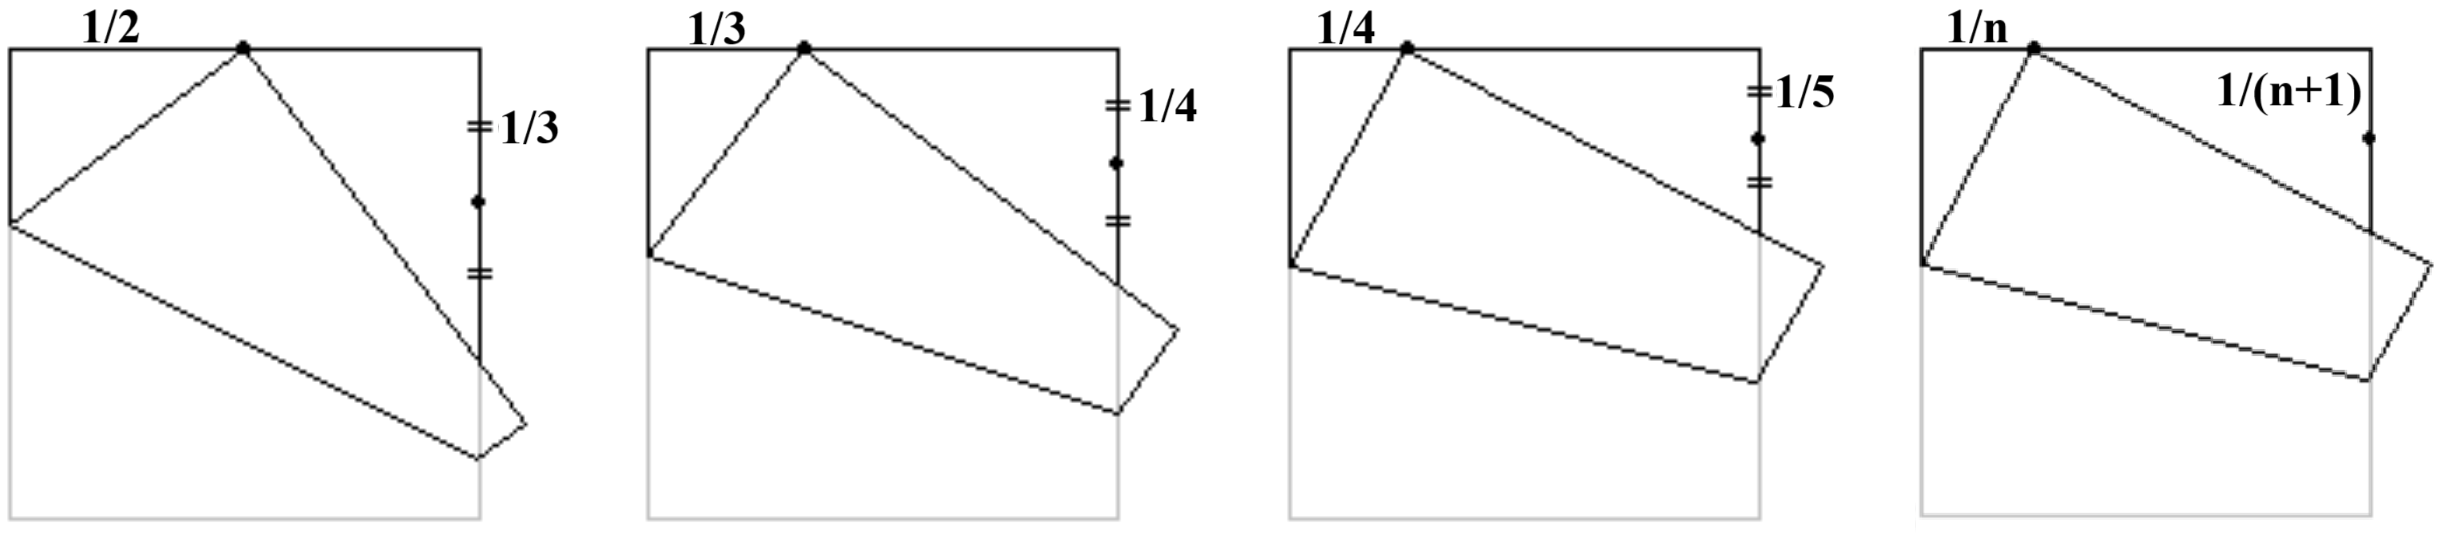
\includegraphics[width=\textwidth]{images/razdelitev_daljice_h1.png}
    \caption[Razdelitev na enake dele (prvi Hagov izrek)]{Konstrukcije razmerij po posplošenem prvem Hagovem izreku.}
    \label{fig:razdelitev_daljice_h1}
\end{figure}

\subsubsection*{Metoda križajočih se diagonal}

Metoda nima uradnega prevoda niti uradnega imena, jo pa tako imenuje Robert J.\ Lang v svojem članku~\cite{lang1988}. Njena konstrukcija je prikazana na sliki~\ref{fig:kriz_diag_3}. Najprej kvadrat dvakrat prepognemo na pol -- enkrat po diagonali skozi oglišči $A$ in $C$ in drugič po vertikali. Nato prepognemo po diagonali (skozi oglišče $B$) še desni pokončen pravokotnik. Presečišče obeh diagonal označimo s točko $P$ in naredimo skoznjo prepogib, ki je pravokoten na horizontalno stranico kvadrata.

\begin{figure}[h]
    \centering
    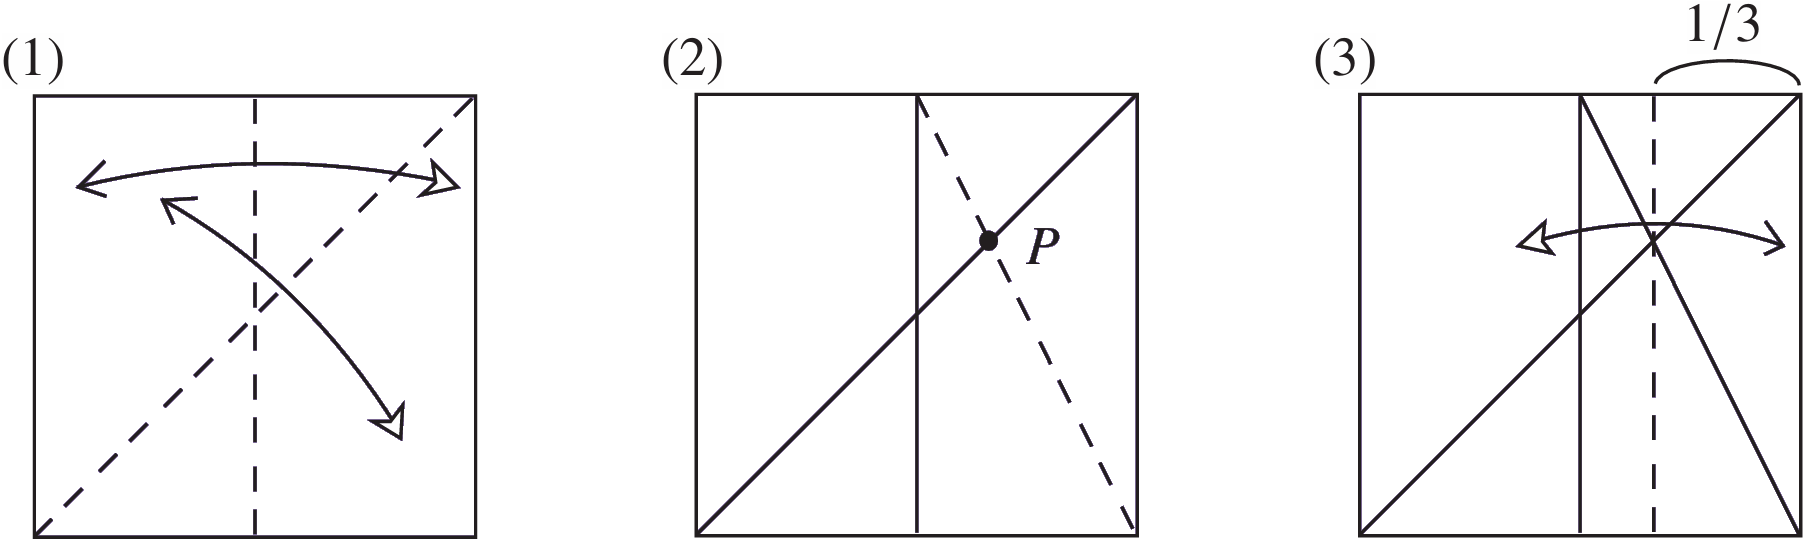
\includegraphics[width=0.9\textwidth]{images/tretjinjenje_stranice1.png}
    \caption[Razdelitev stranice na tri dele]{Konstrukcija po metodi križajoih se diagonal za $n=3$. Preurejeno iz~\cite[str. 37]{hull2013}.}
    \label{fig:kriz_diag_3}
\end{figure}

\begin{trditev}
    \label{trd:kriz_diag_3}
    Zadnji pregib iz zgornjega opisa konstrukcije razdeli horizontalno stranico kvadrata v razmerju $2:1$.
\end{trditev}

\begin{dokaz}
    Dokazujemo lahko na več načinov:
    \begin{enumerate}
        \item \textit{Analitičen pristop:} Kvadrat postavimo v evklidsko ravnino tako, da leži oglišče $A$ v koordinatnem izhodišču in oglišče $B$ v točki $(1, 0)$. Obe diagonali izrazimo z enačbama premic. Glavna diagonala ima enačbo $y = x$, diagonala pravokotnika pa $y = -2x + 2$. Točka $P$ je njuno presečišče in ima tako koordinati $(2/3, 2/3)$.
        \item \textit{Preko podobnih trikotnikov:} Z opisanimi prepogibi v tem kvadratu konstruiramo več trikotnikov. Njihova oglišča označimo tako, kot kaže slika~\ref{fig:kriz_diag_3_dokaz}. Iz podobnosti trikotnikov $\triangle AGP$ in $\triangle ABC$ sledi, da je trikotnik $\triangle AGP$ enakokrak. Naj bo dolžina njegovih krakov $x$. Potem je $|AG| = |GP| = x$ in $|GB| = 1 - x$. Iz podobnosti trikotnikov $\triangle EFB$ in $\triangle PGB$ sledi
        \begin{align*}
            \frac{|EF|}{|FB|} &= \frac{|PG|}{|GB|}, \\
            \frac{1}{\frac{1}{2}} &= \frac{x}{1 - x}, \\
            x &= \frac{2}{3}.
        \end{align*}
    \end{enumerate}
\end{dokaz}
\begin{figure}[h]
    \centering
    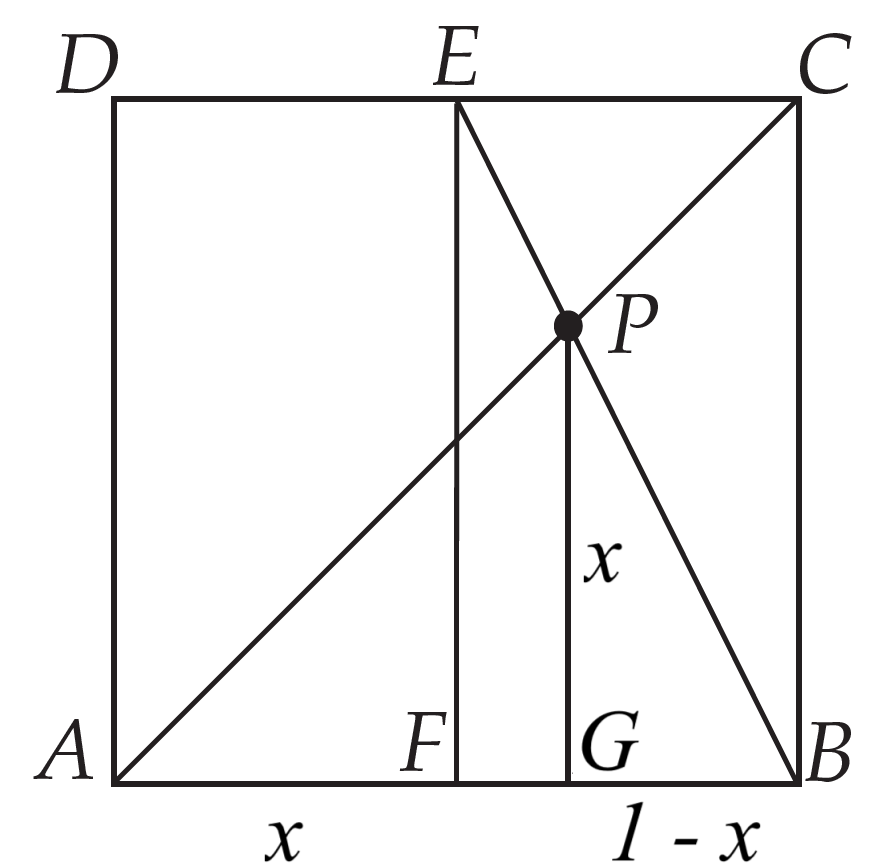
\includegraphics[width=0.3\textwidth]{images/tretjinjenje_stranice2.png}
    \caption[Dokaz metode križajočih diagonal]{Dokaz metode križajočih se diagonal za $n=3$. Preurejeno iz~\cite[str. 38]{hull2013}.}
    \label{fig:kriz_diag_3_dokaz}
\end{figure}

Po konstrukciji pregiba, ki zgornjo stranico kvadrata razdeli v razmerju $2:1$, levi pravokotnik (s stranico $AG$) po vertikali prepognemo še na pol in tako stranico kvadrata razdelimo na tri enake dele. Preidimo sedaj iz $n = 3$ na višje število delov.

Razdelitev stranice kvadrata na štiri dele je že znana -- kvadrat v vertikalni smeri dvakrat prepognemo na pol.

Stranico razdelimo na pet delov na podoben način kot na tri. Naredimo enak pregib po glavni diagonali, nato pa zgornjo stranico razdelimo v razmerju $3:1$ (na primer preko razdelitve na štiri dele). S tem smo na desni strani kvadrata dobili pokončen pravokotnik s horizontalno stranico, dolgo četrt stranice kvadrata. Naslednji pregib je, kot prej, diagonala tega pravokotnika (tista skozi oglišče $B$). Presečišče te in glavne diagonale je točka, ki je od desne stranice oddaljena za $1/5$ (dokaz je analogen tistemu za trditev~\ref{trd:kriz_diag_3}, pri čemer je tu $|FB| = 1/4$ in posledično $x = 4/5$). Naredimo vertikalen pregib skozi točko $P$ in s tem zgornjo stranico kvadrata razdelimo v razmerju $4:1$. Na koncu še levi del te stranice razdelimo na štiri dele. S tem smo celotno stranico razdelili na pet skladnih delov.

Zgornji postopek lahko posplošimo na poljuben $n \in \N$. Kot smo videli v konkretnih primerih za $n = 3$ in $5$, smo si pomagali z vnajprejšnjo razdelitvijo stranice na $n-1$ število enakih delov, kar že znamo storiti. Dokaz naslednje trditve bo tako temeljil na indukciji.

\begin{trditev}[Metoda križajočih se diagonal za splošen $n$]
    Naj bo $n \in \N, n > 2$. Kvadrat $ABCD$ s stranico dolžine $1$ prepognemo po diagonali $AC$, potem pa stranico $DC$ s točko $E$ razdelimo v razmerju $(n-2):1$. Naredimo pregib novonastalega pravokotnika skozi točki $B$ in $E$ (slika~\ref{fig:razdelitev_stranice_n1}). Presečišče te in glavne diagonale je točka $P$, ki je od desne stranice kvadrata oddaljena za $1/n$.
\end{trditev}
\begin{figure}[h]
    \centering
    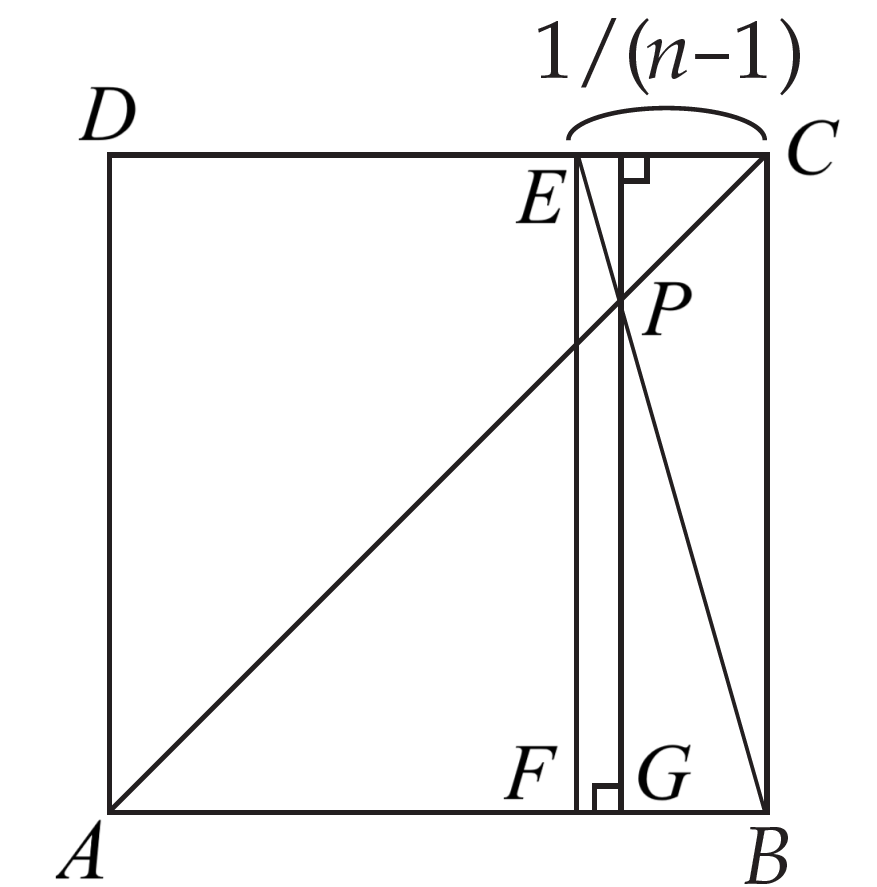
\includegraphics[width=0.3\textwidth]{images/razdelitev_stranice_n1.png}
    \caption[Metoda križajočih diagonal]{Konstrukcija po metodi križajočih se diagonal za splošen $n$. Preurejeno iz~\cite[str. 38]{hull2013}.}
    \label{fig:razdelitev_stranice_n1}
\end{figure}

\begin{dokaz}
    Za $n = 1$ in $n = 2$ ni kaj dokazovati -- v prvem primeru pregiba sploh ni, v drugem primeru stranico prepolovimo.

    \textit{Baza indukcije:} Po trditvi~\ref{trd:kriz_diag_3} že vemo, da trditev drži za $n = 3$ (tudi za $5$).

    \textit{Indukcijska predpostavka:} Predpostavimo, da znamo stranico razdeliti na $n-1$ enakih delov.

    \textit{Indukcijski korak:} Dokazujemo, da znamo stranico razdeliti na $n$ enakih delov. Po navodilih za konstrukcijo iz trditve konstruiramo točko $P$ in pri tem označimo še točke $E, F$ in $G$, kot kaže slika~\ref{fig:razdelitev_stranice_n1}. Potem je dokaz posplošena različica tistega za trditev~\ref{trd:kriz_diag_3}:
    \begin{enumerate}
        \item \textit{Analitičen pristop:} Naj bo oglišče $A$ koordinatno izhodišče in oglišče $B$ točka $(1, 0)$. Premica, ki je nosilka diagonale $AC$, ima tako enačbo $y = x$, nosilka diagonale $CE$ pa $y = -(n-1)x + (n-1)$. Točka $P$ je njuno presečišče in ima tako koordinate $((n-1)/n, (n-1)/n)$. Torej je od desne stranice kvadrata res oddaljena za $1/n$.
        \item \textit{Preko podobnih trikotnikov:} Trikotnik $\triangle AGP$ je enakokrak in naj bo $|AG| = |GP| = x$. Iz razmerij dolžin stranic podobnih trikotnikov $\triangle EFB$ in $\triangle PGB$ sledi
        \begin{align*}
            \frac{|EF|}{|FB|} &= \frac{|PG|}{|GB|}, \\
            \frac{1}{\frac{1}{n-1}} &= \frac{x}{1 - x}, \\
            x &= \frac{n-1}{n}.
        \end{align*}
        Točka $P$ je od desne stranice kvadrata res oddaljena za $1-x = 1/(n + 1)$.
    \end{enumerate}
\end{dokaz}

\begin{posledica}
    Poljubno daljico znamo razdeliti na $n$ skladnih delov za vsak $n \in \N$.
\end{posledica}

\begin{dokaz}
    Vzemimo neko daljico poljubne dolžine. Ker znamo konstruirati pravokotnice skozi točke in prenašati razdalje, lahko konstruiramo kvadrat, katereda zgornja stranica dana daljica. Po zgornji trditvi jo znamo razdeliti v razmerju $(n-1) : 1$ za vsak $n \in \N$. Potem moramo njen daljši del razdeliti na $n-1$ skladnih delov. To storimo na enak način kot prej -- konstruiramo manjši kvadrat s to novo stranico in ponovimo postopek. Ustavimo se, ko na nekem koraku stranico kvadrata razdelimo v razmerju $1:1$ (slika~\ref{fig:razdelitev_daljice_n1}). Takrat bo zgornja stranica oz. dana daljica razdeljena na $n$ skladnih delov.
\begin{figure}[h]
    \centering
    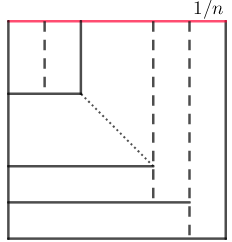
\includegraphics[width=0.3\textwidth]{images/razdelitev_daljice_n1.png}
    \caption[Razdelitev daljice na enake dele]{Razdelitev poljubne stranice (označena z rdečo) na poljubno število skladnih delov.}
    \label{fig:razdelitev_daljice_n1}
\end{figure}
\end{dokaz}

Do zdaj smo imeli metode z razdelitvijo preko prepogibanja kvadratnega lista papirja. Za razdelitev preko pravokotnika je prav tako veliko že razvitih konstrukcij, ki nam njegovo stranico razdelijo na poljubno število skadnih delov. V tej nalogi se s tem ne bomo ukvarjali, bralec pa je povabljen, da si več ogleda v~\cite[str.\ 107--134]{haga2008}.

\subsection{$X$-pregibi}

Poglejmo si še eno zanimivo lastnost, ki jo je odkril Haga in ki izhaja iz prepogibanja kvadrata po principu njegovega prvega izreka (glej~\cite[str.\ 33--44]{haga2008}). Potek konstrukcije je sledeč (slika~\ref{fig:x-pregib_konstr}):
\begin{enumerate}
    \item Na zgornji stranici kvadrata izberemo poljubno točko.
    \item Levo spodnje oglišče prepognemo na izbrano točko.
    \item Papir razgrnemo in opazimo pregib.
    \item Nato na izbrano točko prepognemo še desno spodnje oglišče.
    \item Papir razgnemo in opazimo nov pregib.
\end{enumerate}

\begin{figure}[h]
    \centering
    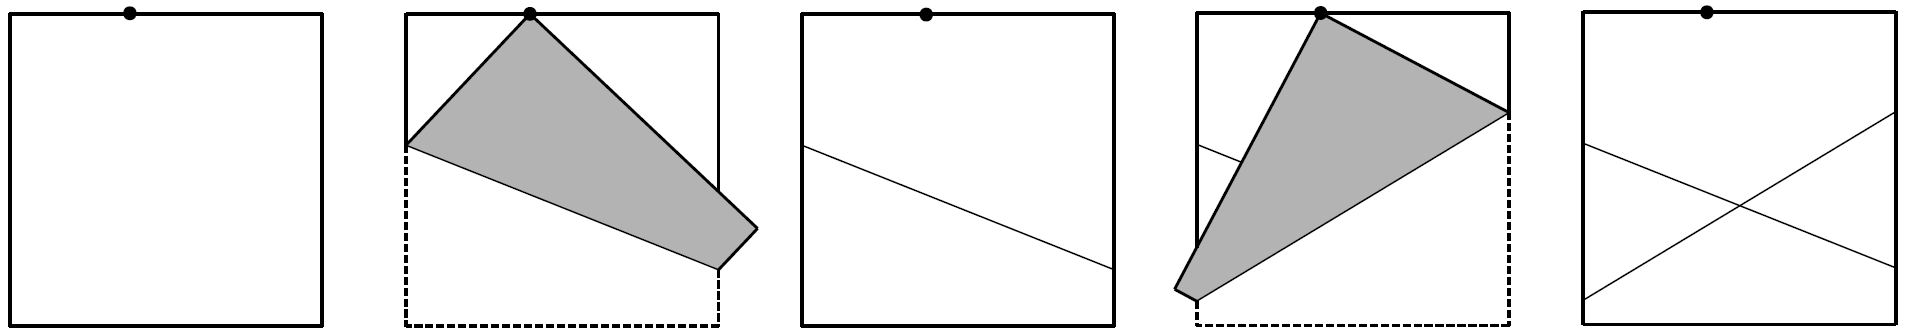
\includegraphics[width=\textwidth]{images/x-pregibi/konstrukcija.png}
    \caption[Konstrukcija $X$-pregibov]{Potek konstrukcije $X$-pregibov. Predelano iz~\cite[str.\ 34]{haga2008}.}
    \label{fig:x-pregib_konstr}
\end{figure}

Par pregibov, ki smo ju dobili po opravljenem postopku, po videzu spominja na črko $X$, zato ju avtor imenuje kar \emph{$X$-pregiba}.

Bralec je povabljen, da za več razliščnih točk na zgornji stranici kvadrata opravi pripadajoče $X$-pregibe. Nato pa naj kvadrat prepogne še na pol po vertikali. Mogoče ga bo presenetilo, da le-ta vedno poteka skozi presečišče $X$-pregibov!

V resnici to ni težko dokazati. Uvedimo najprej oznake točk, kot kaže slika~\ref{fig:x-pregib_dokaz}. Pri tem je $E$ poljubna izbrana točka, gledamo pa trikotnik $\triangle BCE$.
\begin{figure}[h]
    \centering
    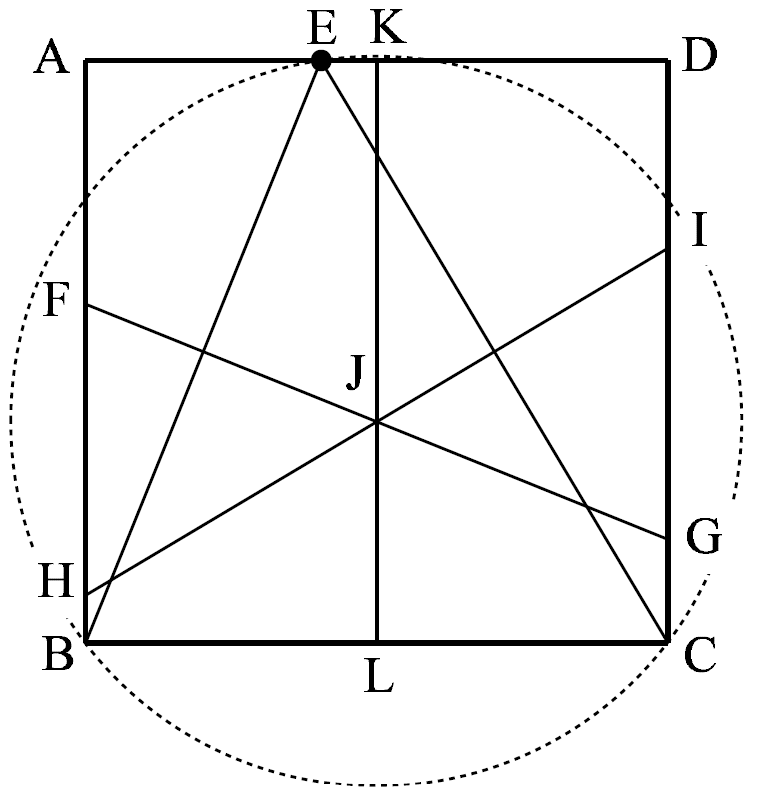
\includegraphics[width=0.35\textwidth]{images/x-pregibi/dokaz_presecisca.png}
    \caption[Dokaz presečišča $X$-pregibov]{Dokaz, da se $X$-pregiba in navpična simetrala kvadrata sekajo v isti točki. Vzeto iz~\cite[str.\ 38]{haga2008}.}
    \label{fig:x-pregib_dokaz}
\end{figure}
Po konstrukciji je pregib $FG$ po konstrukciji simetrala njegove stranice $BE$, pregib $HI$ simetrala stranice $CE$ in pregib $KL$ simetrala stranice $BC$ in hkrati navpična simetrala kvadrata $ABCD$. Vemo, da se simetrale stranic trikotnika sekajo v skupni točki, torej smo s tem še matematično potrdili zgornjo opazko iz konstrukcije.

Naj bo $J$ presečišče simetral stranic trikotnika $\triangle BCE$. Potem je to hkrati tudi središče njegove očrtane krožnice, kot je načrtana na sliki~\ref{fig:x-pregib_dokaz}. Posledično so seveda razdalje oglišč $B, C$ in $E$ do točke $J$ polmeri krožnice, torej so med seboj skladne.

Bralec naj sedaj vzame vse svoje kvadratne liste papirja, na katere je konstruiral različne $X$-pregibe, in jih zloži drug na drugega. Opazka, da presečišča pregibov ležijo na isti premici, ni presenetljiva, saj smo ravnokar premislili, da vsako tako presečišče leži na navpični simetrali kvadrata. Bolj je zanimiva opazka, da nobeno od teh presečišč ne leži v zgornji polovici kvadrata (slika~\ref{fig:x-pregib_primeri_skup}).

\begin{figure}[h]
    \centering
    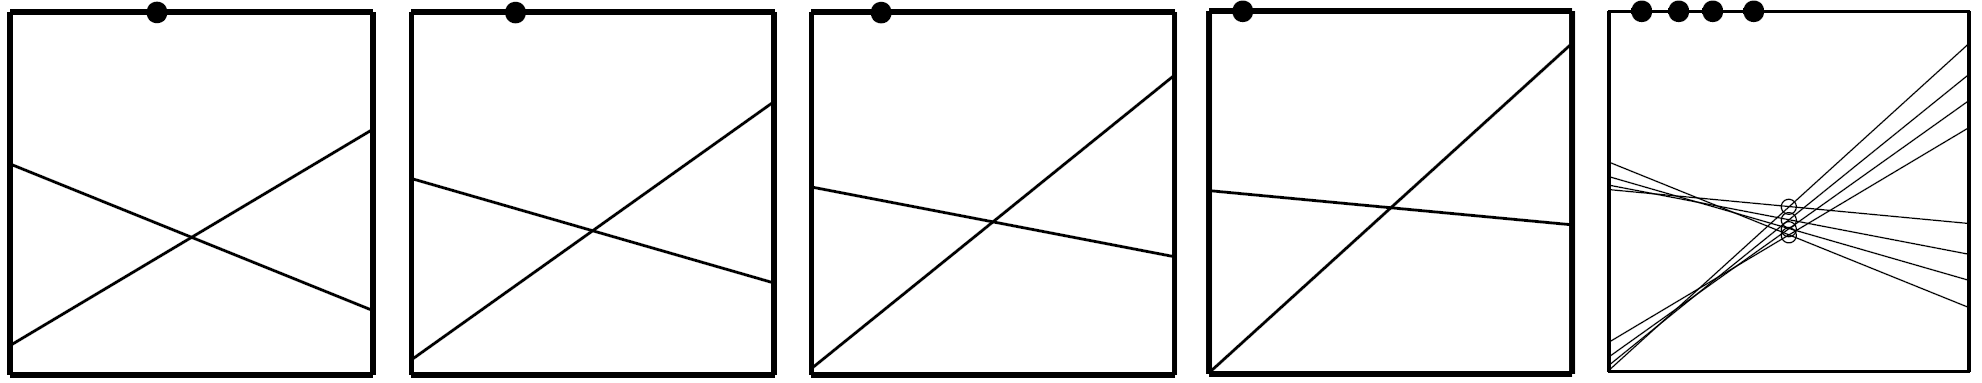
\includegraphics[width=0.9\textwidth]{images/x-pregibi/primeri_skupaj.png}
    \caption[Primeri $X$-pregibov]{Primeri $X$-prepogibov in njihova unija. Predelano iz~\cite[str.\ 36]{haga2008}.}
    \label{fig:x-pregib_primeri_skup}
\end{figure}

Kvadrat lahko postavimo v koordinatni sistem z ogliščem $B$ v izhodišču in ogliščem $A$ v točki $(0,1)$. Če naj bo $E = (a, 1)$ poljubna točka na stranici $AD$. Ohranimo oznake točk s slike~\ref{fig:x-pregib_dokaz}. Premici, ki predstavljata $X$-pregiba $FG$ in $HI$, imata enačbi
$$ y_{FG} = -ax + \frac{a^2}{2} + \frac{1}{2} \; \text{ in } \; y_{HI} = (1-a)x + \frac{a^2}{2}. $$
Njuno presečišče je točka $J$, katere abscisa je $1/2$ po konstrukciji. Vstavimo to v eno izmed enačb premic in dobimo še njeno ordinato, ki je odvisna od $a$:
$$ y_J(a) = \frac{1}{2} \left(a - \frac{1}{2}\right)^2 + \frac{3}{8}. $$
Ker velja $a \in [0,1]$, je ordinata točke $J$ omejena z $3/8 \leq y_J \leq 1/2$. Na sliki~\ref{fig:x-pregib_visina_pres} je levo je prikazan graf funkcije $y_J(a)$, na desni pa primerjava ordinat presečišča $J$ glede na izbran $a$. Najnižja vrednost je dosežena pri $a = 1/2$, torej če za točko $E$ izberemo središče daljice $AD$, najvišja pa pri $a \in \{0, 1\}$, torej pri izbiri oglišč $A$ oziroma $D$.
\begin{figure}[h]
    \centering
    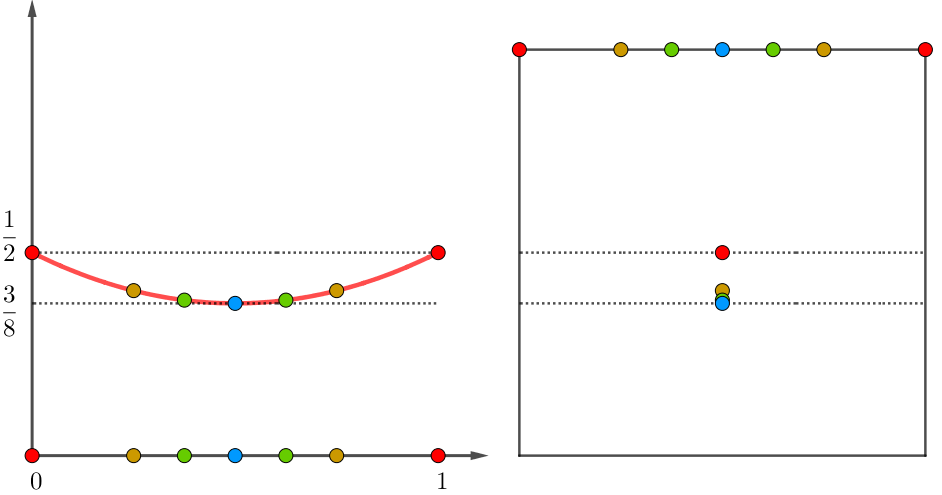
\includegraphics[width=0.5\textwidth]{images/x-pregibi/visina_presecisca.png}
    \caption[Višina presečišča $X$-pregibov]{Višina presečišča $X$-pregibov glede na absciso izbrane točke $E$.}
    \label{fig:x-pregib_visina_pres}
\end{figure}

Tu še ni konec -- poglejmo si trikotnika $\triangle FHJ$ in $\triangle GIJ$ (slika~\ref{fig:x-pregib_dokaz_odsek}). Ker imata enak kot v vrhu $J$ in sta osnovnici vzporedni, sta podobna, ker pa točka $J$ razpolavlja pregiba $FG$ in $HI$, sta celo skladna, torej $|FH| = |GI|$. Ker sta kraka kotov $\angle HFJ$ in $\angle CBE$ paroma pravokotna, sta kota skladna. Na enak način se prepričamo še o skladnosti kotov $\angle GIJ$ in $\angle BCE$. Torej je trikotnik $\triangle BCE$ podoben trikotnikoma $\triangle FHJ$ in $\triangle GIJ$.
\begin{figure}[h]
    \centering
    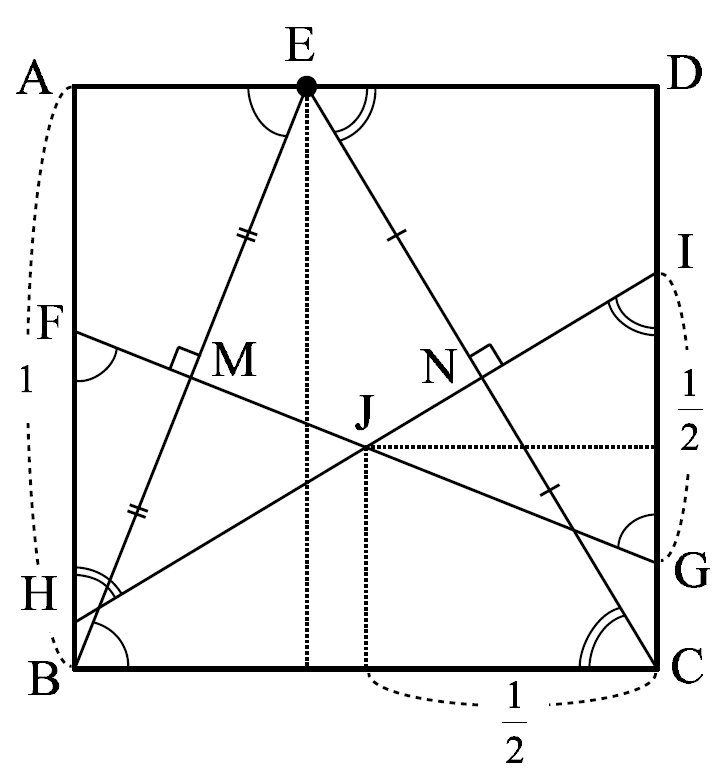
\includegraphics[width=0.35\textwidth]{images/x-pregibi/dokaz_odseki.png}
    \caption[Dokaz za dolžini odsekov $X$-pregibov]{Dokaz, da $X$-pregiba na vertikalnih stranicah kvadrata odrežeta enaka odseka. Vzeto iz~\cite[str.\ 41]{haga2008}.}
    \label{fig:x-pregib_dokaz_odsek}
\end{figure}
Ker je v trikotniku $\triangle BCE$ njegova višina enako dolga kot osnovnica, to velja tudi za ostala trikotnika. Njuna višina je (ker točka $J$ leži na navpični simetrali kvadrata $ABCD$) enaka $1/2$, torej velja
$$ |FH| = |GI| = \frac{1}{2}. $$

Haga lastnosti $X$-pregibov raziskuje tudi na pravokotnikih. Izkaže se, da zanje veljajo enake lastnosti razen zadnje -- z daljšanjem daljše stranice pravokotnika se namreč (sicer še vedno skladni) daljici $FH$ in $GI$ vedno krajšata. Matematični premislek prepuščamo bralcu, je pa zelo podoben temu za kvadratno različico (slika~\ref{fig:x-pregib_dokaz_pravokotnik}).

\begin{figure}[h]
    \centering
    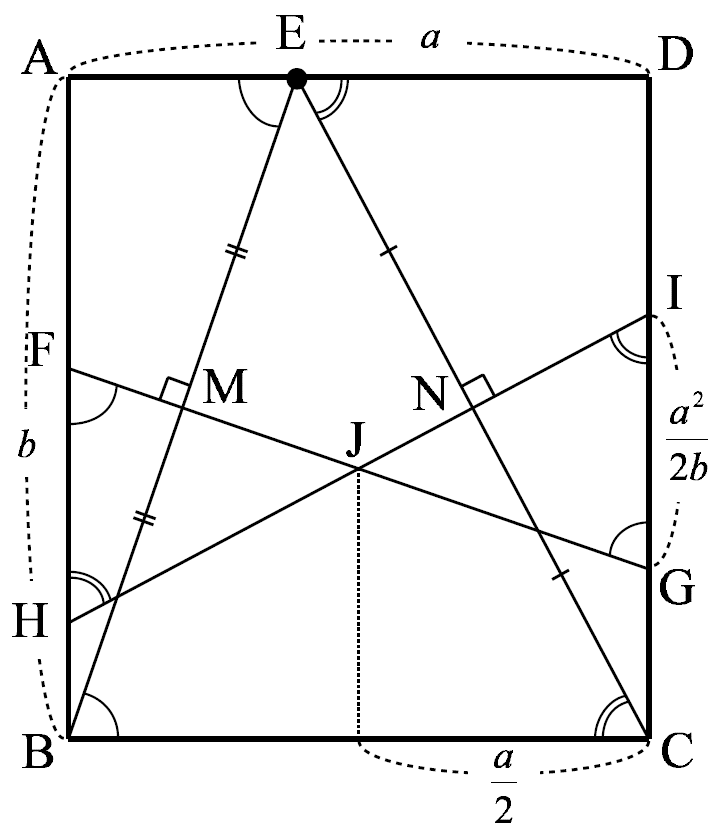
\includegraphics[width=0.35\textwidth]{images/x-pregibi/dokaz_pravokotnik.png}
    \caption[$X$-pregiboa v pravokotniku]{$X$-pregiba v pravokotniku. Vzeto iz~\cite[str.\ 44]{haga2008}.}
    \label{fig:x-pregib_dokaz_pravokotnik}
\end{figure}